% Versão 24/06/2020

% Este documento destina-se a servir como modelo para a produção de documentos
% de pesquisa do PPGINF/UFPR, como projetos, dissertações e teses. A classe de
% documento se chama "ppginf" (arquivo ppginf.cls) e define o formato básico do
% documento. O texto está organizado em capítulos que são colocados em
% subdiretórios separados. São definidos exemplos para a inclusão de figuras,
% códigos-fonte e a definição de tabelas.
%
% Produzido por Carlos Maziero (maziero@inf.ufpr.br).

%=====================================================

% Opções da classe ppginf:
%
% - defesa    : versão para entregar à banca; tem espaçamento 1,5
%               e omite algumas páginas iniciais (agradecimentos, etc)
% - final     : versão pós-defesa, para enviar à biblioteca;
%               tem espaçamento simples e todas as páginas iniciais.
% - oneside   : somente frente; use quando for gerar somente o PDF.
% - twoside   : frente/verso; use se precisar de uma versão impressa.
% - metadados : inclui metadados no PDF (por default não inclui)
% - ...       : demais opções aceitas pela classe "book"

% ATENÇÂO: este modelo tem suporte para português e inglês.
% As duas línguas devem ser informadas como opção da classe;
% a língua principal do documento deve vir POR ÚLTIMO.

% Versão de defesa em português
\documentclass[defesa,oneside,english,brazilian]{ppginf}

% Versão de defesa em inglês
%\documentclass[defesa,oneside,brazilian,english]{ppginf}

% Versão final em PDF para a biblioteca da UFPR (português e inglês)
%\documentclass[final,oneside,english,brazilian]{ppginf}
%\documentclass[final,oneside,brazilian,english]{ppginf}

% Versão final para impressão (frente/verso)
%\documentclass[final,twoside,english,brazilian]{ppginf}

% configurações de diversos pacotes, inclusive a fonte usada no texto
% Pacotes usados neste documento e suas respectivas configurações

% ------------------------------------------------------------------------------

% Definição de fontes

% formato dos arquivos-fonte (utf8 no Linux e latin1 no Windows)
\usepackage[utf8]{inputenc}	% arquivos LaTeX em Unicode (UTF8)

% usar codificação T1 para ter caracteres acentuados corretos no PDF
\usepackage[T1]{fontenc}

% fonte usada no corpo do texto (pode alterar, mas descomente apenas uma)
\usepackage{newtxtext,newtxmath}	% Times (se não tiver, use mathptmx)
%\usepackage{lmodern}			% Computer Modern (fonte clássico LaTeX)
%\usepackage{kpfonts}			% Kepler/Palatino (idem, use mathpazo)
%\renewcommand{\familydefault}{\sfdefault} % Arial/Helvética (leia abaixo)

% A biblioteca central da UFPR recomenda usar Arial, seguindo a recomendação da
% ABNT. Essa é uma escolha ruim, pois fontes sans-serif são geralmente inade-
% quados para textos longos e impressos, sendo melhores para páginas Web.
% http://www.webdesignerdepot.com/2013/03/serif-vs-sans-the-final-battle/.

% fontes usadas em ambientes específicos
\usepackage[scaled=0.9]{helvet}		% Sans Serif
\usepackage{courier}			% Verbatim, Listings, etc

% ------------------------------------------------------------------------------

% inclusão de figuras em PDF, PNG, PS, EPS
\usepackage{graphicx}

% subfiguras (subfigure is deprecated, don't use it)
\usepackage[labelformat=simple]{subcaption}
\renewcommand\thesubfigure{(\alph{subfigure})}

% ------------------------------------------------------------------------------

% inclusão/formatação de código-fonte (programas)
\usepackage{listings}
\lstset{language=c}
\lstset{basicstyle=\ttfamily\footnotesize,commentstyle=\textit,stringstyle=\ttfamily}
\lstset{showspaces=false,showtabs=false,showstringspaces=false}
\lstset{numbers=left,stepnumber=1,numberstyle=\tiny}
\lstset{columns=flexible,mathescape=true}
\lstset{frame=single}
\lstset{inputencoding=utf8,extendedchars=true}
\lstset{literate={á}{{\'a}}1  {ã}{{\~a}}1 {à}{{\`a}}1 {â}{{\^a}}1
                 {Á}{{\'A}}1  {Ã}{{\~A}}1 {À}{{\`A}}1 {Â}{{\^A}}1
                 {é}{{\'e}}1  {ê}{{\^e}}1 {É}{{\'E}}1  {Ê}{{\^E}}1
                 {í}{{\'\i}}1 {Í}{{\'I}}1
                 {ó}{{\'o}}1  {õ}{{\~o}}1 {ô}{{\^o}}1
                 {Ó}{{\'O}}1  {Õ}{{\~O}}1 {Ô}{{\^O}}1
                 {ú}{{\'u}}1  {Ú}{{\'U}}1
                 {ç}{{\c{c}}}1 {Ç}{{\c{C}}}1 }

% ------------------------------------------------------------------------------

% formatação de algoritmos
\usepackage{algorithm,algorithmic}
\IfLanguageName{brazilian} {\floatname{algorithm}{Algoritmo}}{}
\renewcommand{\algorithmiccomment}[1]{~~~// #1}
%\algsetup{linenosize=\footnotesize,linenodelimiter=.}

% ------------------------------------------------------------------------------

% formatação de bibliografia
\usepackage{natbib}			% bibliografia no estilo NatBib
\IfLanguageName{brazilian}
{\bibliographystyle{apalike-ptbr}}	% formato em português
{\bibliographystyle{apalike}}		% formato em inglês

% Estilos de bibliografia recomendados (só descomentar um estilo!)
% Mais infos: https://pt.sharelatex.com/learn/Bibtex_bibliography_styles
%
%\bibliographystyle{apalike-ptbr}	% [Maziero et al., 2006]
%\bibliographystyle{alpha}		% [Maz06]
%\bibliographystyle{plainnat}		% vide Google "LaTeX Natbib"
%\bibliographystyle{plain}		% [1] ordem alfabética
%\bibliographystyle{unsrt}		% [1] ordem de uso no texto

% no estilo "unsrt", evita que citações nos índices sejam consideradas
%\usepackage{notoccite}

\renewcommand{\cite}{\citep}	% \cite deve funcionar como \citep
%\bibpunct{[}{]}{;}{a}{}{,}	% caracteres usados nas referências

% ------------------------------------------------------------------------------

% fontes adicionais
\usepackage{amsmath}		% pacotes matemáticos
\usepackage{amsfonts}		% fontes matemáticas 
%\usepackage{amssymb}		% símbolos 

% ------------------------------------------------------------------------------

% pacotes diversos
\usepackage{alltt,moreverb}	% mais comandos no modo verbatim
\usepackage{lipsum}		% gera texto aleatório (para os exemplos)
\usepackage{currfile}		% infos sobre o arquivo/diretório atual
\usepackage[final]{pdfpages}	% inclusão de páginas em PDF
\usepackage{longtable}		% tabelas multi-páginas (tab símbolos/acrônimos)

% ------------------------------------------------------------------------------



%=====================================================

\begin {document}

% Principais dados, usados para gerar as páginas iniciais.
% Campos não utilizados podem ser removidos ou comentados.

% título
\title{Teste Wald para estudo de parâmetros de modelos multivariados de covariância linear generalizada}

% palavras-chave e keywords (p/ resumo, abstract e metadados do PDF)
\pchave{Palavra-chave 1. Palavra-chave 2. Palavra-chave 3.}
\keyword{Keyword 1. Keyword 2. Keyword 3.}

% autoria
\author{Lineu Alberto Cavazani de Freitas}
\advisor{Prof. Dr. Wagner Hugo Bonat}
\coadvisor{Prof. Dr. Marco Antônio Zanata Alves}

% instituição
\IfLanguageName{brazilian}
  { \instit{UFPR}{Universidade Federal do Paraná} }
% a Bib/UFPR exige que tudo seja em português, exceto o título :-(
%  { \instit{UFPR}{Federal University of Paraná} }
  { \instit{UFPR}{Universidade Federal do Paraná} }

% área de concentração (default do PPGInf, não mudar)
\IfLanguageName{brazilian}
  { \field{Ciência da Computação} }
% a Bib/UFPR exige que tudo seja em português, exceto o título :-(
%  { \field{Computer Science} }
  { \field{Ciência da Computação} }

% data (só o ano)
\date{2021}

% local
\IfLanguageName{brazilian}
  { \local{Curitiba PR} }
% a Bib/UFPR exige que tudo seja em português, exceto o título :-(
%  { \local{Curitiba PR - Brazil} }
  { \local{Curitiba PR} }

% imagem de fundo da capa (se não desejar, basta comentar)
\coverimage{0-iniciais/fundo-capa.jpg}

%=====================================================

%% Descrição do documento (obviamente, descomentar somente UMA!)

% Por exigência da biblioteca da UFPR, a descrição do documento deve ser
% em português, mesmo em documentos em outras línguas. Vá entender...

% tese de doutorado
%\descr{Tese apresentada como requisito parcial à obtenção do grau de Doutor em Ciência da Computação no Programa de Pós-Graduação em Informática, Setor de Ciências Exatas, da Universidade Federal do Paraná}

% exame de qualificação de doutorado
%\descr{Documento apresentado como requisito parcial ao exame de qualificação de Doutorado no Programa de Pós-Graduação em Informática, Setor de Ciências Exatas, da Universidade Federal do Paraná}

% dissertação de mestrado
\descr{Dissertação apresentada como requisito parcial à obtenção do grau de Mestre em Informática no Programa de Pós-Graduação em Informática, Setor de Ciências Exatas, da Universidade Federal do Paraná}

% exame de qualificação de mestrado
%\descr{Documento apresentado como requisito parcial ao exame de qualificação de Mestrado no Programa de Pós-Graduação em Informática, Setor de Ciências Exatas, da Universidade Federal do Paraná}

% trabalho de conclusão de curso
%\descr{Trabalho apresentado como requisito parcial à conclusão do Curso de Bacharelado em XYZ, Setor de Ciências Exatas, da Universidade Federal do Paraná}

% trabalho de disciplina
%\descr{Trabalho apresentado como requisito parcial à conclusão da disciplina XYZ no Curso de Bacharelado em XYZ, Setor de Ciências Exatas, da Universidade Federal do Paraná}

% doctorate thesis
%\descr{Thesis presented as a partial requirement for the degree of Doctor in Computer Science in the Graduate Program in Informatics, Exact Sciences Sector, of the Federal University of Paraná, Brazil}

% doctorate qualification
%\descr{Document presented as a partial requirement for the doctoral qualification exam in the Graduate Program in Informatics, Exact Sciences Sector, of the Federal University of Paraná, Brazil}

% MSc dissertation
%\descr{Dissertation presented as a partial requirement for the degree of Master of Sciences in Informatics in the Graduate Program in Informatics, Exact Sciences Sector, of the Federal University of Paraná, Brazil.}

% MSc qualification
%\descr{Document presented as a partial requirement for the Master of Sciences qualification exam in the Graduate Program in Informatics, Exact Sciences Sector, of the Federal University of Paraná, Brazil}

%=====================================================

% define estilo das páginas iniciais (capas, resumo, sumário, etc)
\frontmatter
\pagestyle{frontmatter}

% produz capa e folha de rosto
\titlepage

% páginas que só aparecem na versão final (a inclusão é automática)
% IMPORTANTE: o conteúdo exato da ficha catalográfica é preparada pela
% Biblioteca da UFPR. Não "invente" um conteúdo para ela!

\begin{ficha}	% só gera conteúdo se for na versão final

% inclusão da ficha catalográfica final (arquivo PDF)
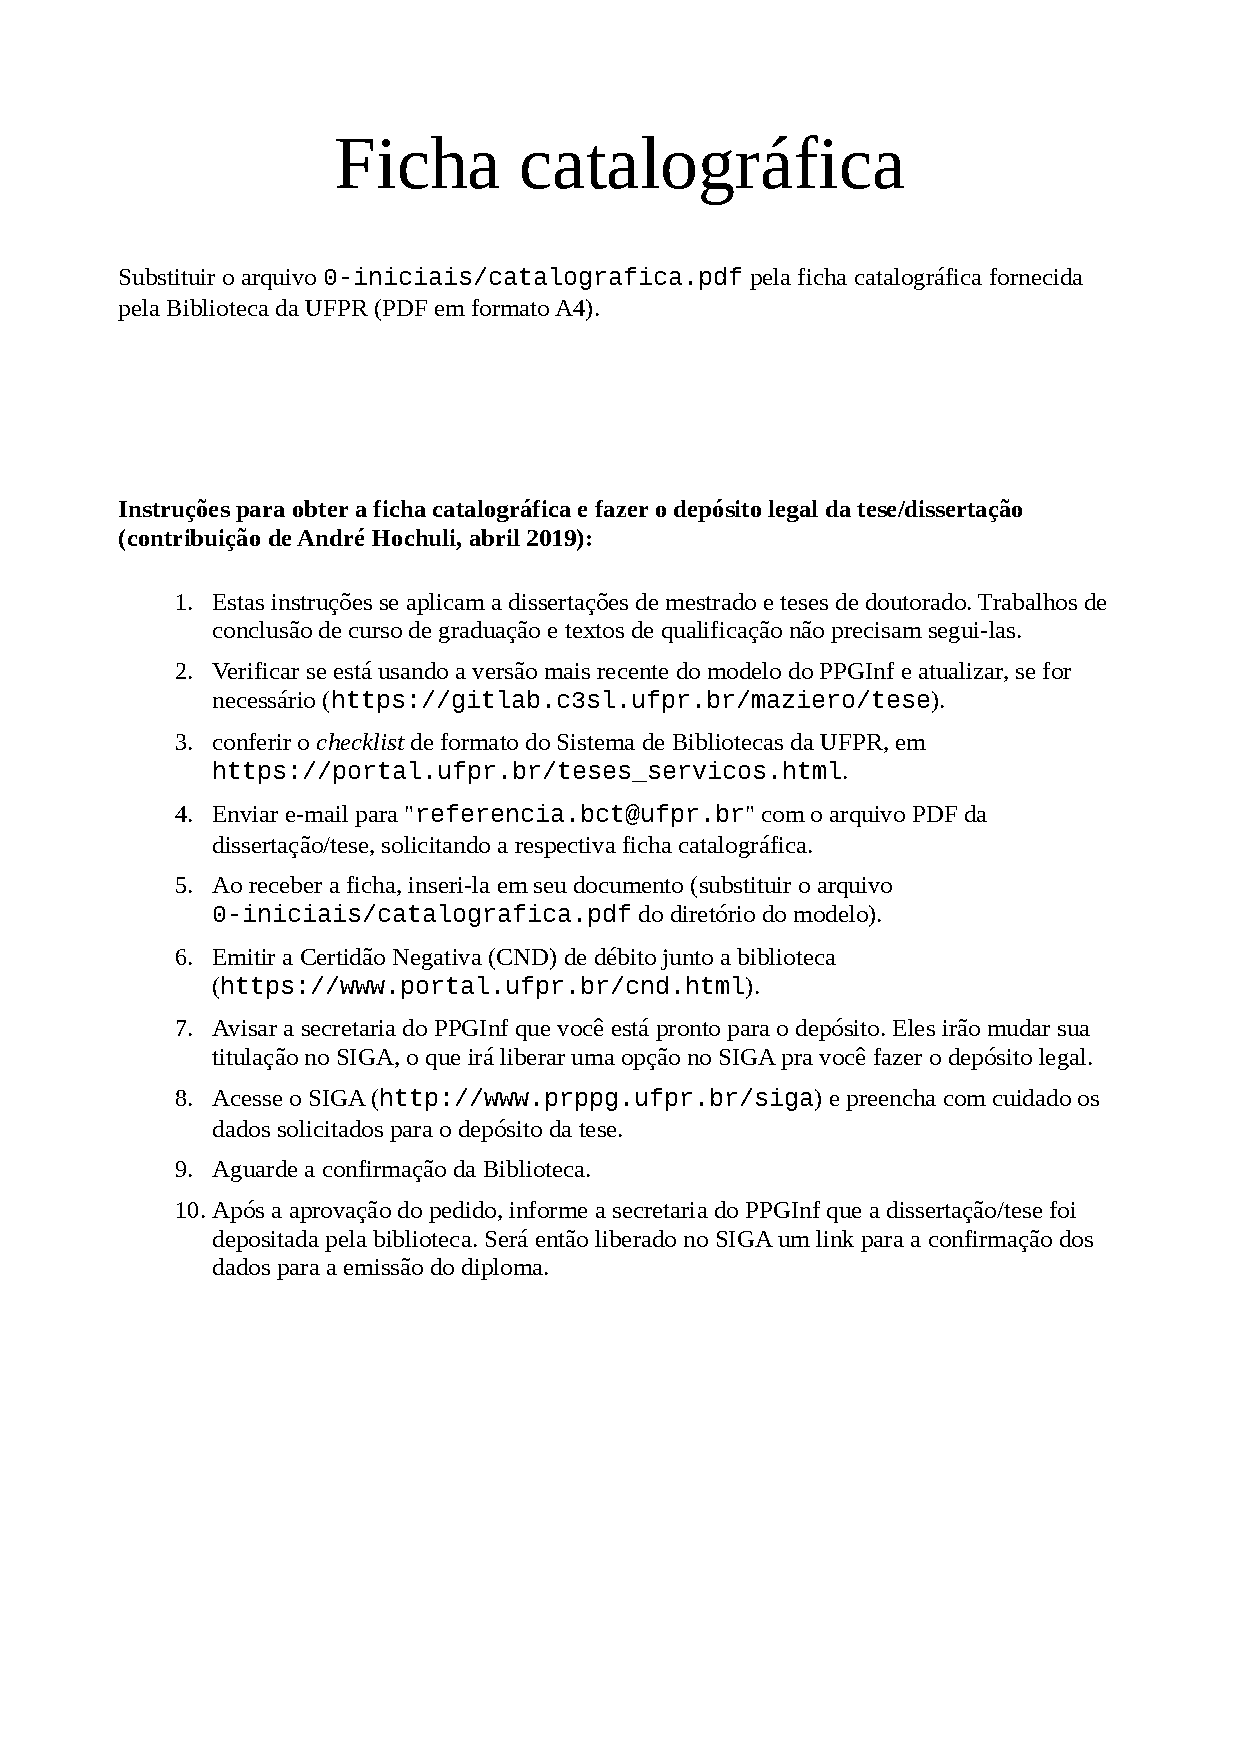
\includepdf[noautoscale]{0-iniciais/catalografica.pdf}

\end{ficha}

%=====================================================
	% ficha catalográfica
% A ficha de aprovação será fornecida pela secretaria do programa,
% após a defesa e cumprimento dos demais trâmites legais.

\begin{aprovacao}	% só gera conteúdo se for na versão final

% inclusão do termo de aprovação final (arquivo PDF)
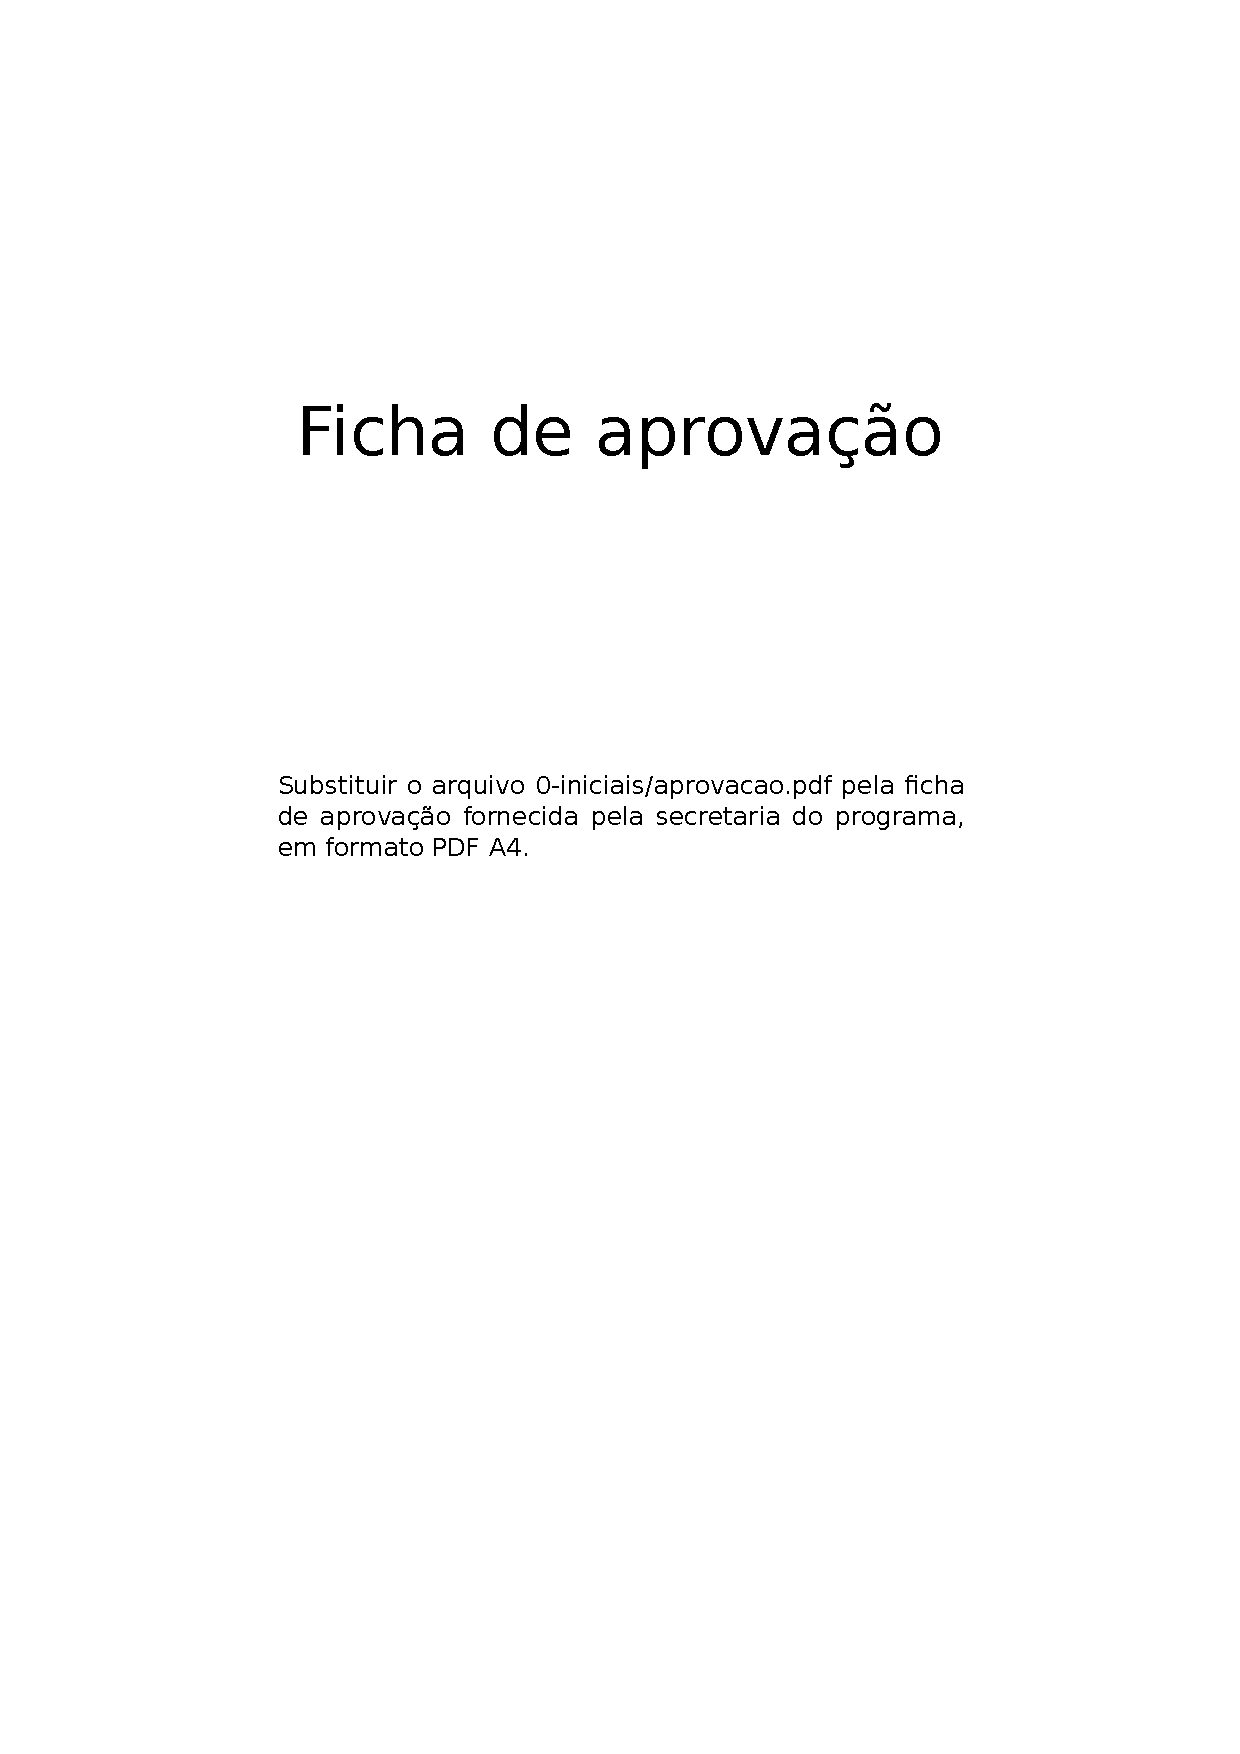
\includepdf[noautoscale]{0-iniciais/aprovacao.pdf}

\end{aprovacao}

%=====================================================
		% folha de aprovação
\begin{dedica}  % só gera conteúdo se for na versão final

A alguém...

\end{dedica}

		% dedicatória
\begin{agradece}	% só gera conteúdo se for na versão final

Inserir os agradecimentos. Os agradecimentos devem ocupar no máximo uma página, devem ser justificados na largura da página e com um afastamento de parágrafo na primeira linha de 1,27 cm. O espaçamento entre linhas deve ser de 1,5 linhas. Não deve haver espaçamento adicional entre parágrafos.

\lipsum[2-5]	% gera um texto aleatório

\end{agradece}

		% agradecimentos

% resumo (português) e abstract (inglês)
\begin{resumo}

O resumo deve conter no máximo 500 palavras, devendo ser justificado na largura da página e escrito em um único parágrafo\footnote{E também não deve ter notas de rodapé; em outras palavras, não siga este exemplo... ;-)} com um afastamento de 1,27 cm na primeira linha. O espaçamento entre linhas deve ser de 1,5 linhas. O resumo deve ser informativo, ou seja, é a condensação do conteúdo e expõe finalidades, metodologia, resultados e conclusões.

\lipsum[10-13]	% texto aleatório

\end{resumo}

\begin{abstract}

The abstract should be the English translation of the ``resumo'', no more, no less.

\lipsum[10-13]	% texto aleatório

\end{abstract}


% listas  de figuras, tabelas, abreviações/siglas, símbolos
\listoffigures				% figuras
\clearpage
\listoftables				% tabelas
%=====================================================

% lista de acrônimos (siglas e abreviações)

\begin{listaacron}

\begin{longtable}[l]{p{0.2\linewidth}p{0.7\linewidth}}

LM & Modelo linear\\
GLM & Modelo linear generalizado\\
cGLM & Modelo de covariância linear generalizada\\
McGLM & Modelo multivariado de covariância linear generalizada\\
ANOVA & Análise de variância\\
MANOVA & Análise de variância multivariada\\

\end{longtable}

\end{listaacron}

%=====================================================
		% acrônimos, deve ser preenchida à mão
%=====================================================

% lista de símbolos

\begin{listasimb}

\begin{longtable}[l]{p{0.2\linewidth}p{0.7\linewidth}}
$\alpha$ & alfa, primeira letra do alfabeto grego\\
$\beta$ & beta, segunda letra do alfabeto grego\\
$\gamma$ & gama, terceira letra do alfabeto grego\\
$\omega$ & ômega, última letra do alfabeto grego\\
$\pi$ & pi \\
$\tau$ & Tempo de resposta do sistema\\
$\theta$ & Ângulo de incidência do raio luminoso\\
\end{longtable}

\end{listasimb}

%=====================================================
		% símbolos, idem
\tableofcontents			% sumário

%=====================================================

% define estilo do corpo do documento (capítulos e apêndices)
\mainmatter
\pagestyle{mainmatter}

% inclusao de cada capítulo, alterar a gosto (do professor de Metodologia)
\chapter{Introdução}

%=====================================================

\section{Motivação}

% CIENCIA DE DADOS

Desde o surgimento do termo \emph{data science} por volta de 1996 \citep{histds} a discussão sobre o tema atrai pesquisadores das mais diversas áreas \citep{cao2016data}. A ciência de dados é vista como um campo de estudo de natureza interdisciplinar que incorpora conhecimento de grandes áreas como estatística, ciência da computação e matemática \citep{ley2018makes}. \citet{weihs2018data} afirmam que a ciência de dados é um campo em muito influenciado por áreas como informática, ciência da computação, matemática, pesquisa operacional, estatística e ciências aplicadas. Em \citet{cao2016data} é dito que ciência de dados engloba técnicas de como: estatística, aprendizado de máquina, gerenciamento de \emph{big data}, dentre outras. 

Alguns dos campos de interesse da ciência de dados são: métodos de amostragem, mineração de dados, bancos de dados, técnicas de análise exploratória, probabilidade, inferência, otimização, infraestrutura computacional, plataformas de \emph{big data}, modelos estatísticos, dentre outros. \citet{weihs2018data} afirmam que os métodos estatísticos são de fundamental importância em grande parte das etapas da ciência de dados. Neste sentido, os modelos de regressão tem papel importante. Tais modelos são indicados a problemas nos quais existe interesse em verificar a associação entre uma ou mais variáveis resposta (também chamadas de variáveis dependentes) e um conjunto de variáveis explicativas (também chamadas de variáveis independentes, covariáveis ou preditoras).

% MODELOS DE REGRESSAO

Para entender minimamente um modelo de regressão, é necessário compreender o conceito de fenômeno aleatório, variável aleatória e distribuição de probabilidade. Um fenômeno aleatório é uma situação na qual diferentes observações podem fornecer diferentes desfechos. Estes fenômenos podem ser descritos por variáveis aleatórias que associam um valor numérico a cada desfecho possível do fenômeno. Os desfechos deste fenômeno podem ser descritos por uma escala que pode ser discreta ou contínua. Uma variável aleatória é considerada discreta quando os possíveis desfechos estão dentro de um conjunto enumerável de valores. Já uma variável aleatória contínua ocorre quando os possíveis resultados estão em um conjunto não enumerável de valores. Na prática existem probabilidades associadas aos valores de uma variável aleatória, e estas probabilidades podem ser descritas por meio de funções. No caso das variáveis discretas, a função que associa probabilidades aos valores da variável aleatória é chamada de função de probabilidade. No caso das contínuas, esta função é chamada de função densidade de probabilidade.

Existem ainda modelos probabilísticos que buscam descrever as probabilidades de variáveis aleatórias: as chamadas distribuições de probabilidade. Portanto, em problemas práticos, podemos buscar uma distribuição de probabilidades que melhor descreva o fenômeno de interesse. Estas distribuições são descritas por funções e tais funções possuem parâmetros que controlam aspectos da distribuição como escala e forma, sendo que estes parâmetros são quantidades desconhecidas estimadas por meio dos dados. Na análise de regressão busca-se modelar os parâmetros das distribuições de probabilidade como uma função de outras variáveis. Isto é feito por meio da decomposição do parâmetro da distribuição em outros parâmetros, chamados de parâmetros de regressão, que dependem de variáveis conhecidas e fixas: as variáveis explicativas.  

Assim, o objetivo dos modelos de regressão consiste em obter uma equação que explique a relação entre as variáveis explicativas e o parâmetro de interesse da distribuição de probabilidades selecionada para modelar a variável aleatória. Em geral, o parâmetro de interesse da distribuição de probabilidades modelado em função das variávis explicativas é a média. Fazendo uso da equação resultante do processo de análise de regressão, é possível estudar a importância das variáveis explicativas sobre a resposta e realizar predições da variável resposta com base nos valores observados das variáveis explicativas. 

Em contextos práticos o processo de análise via modelo de regressão parte de um conjunto de dados. Neste contexto, um conjunto de dados é uma representação tabular em que unidades amostrais são representadas nas linhas e seus atributos (variáveis) são representados nas colunas. Pode-se usar um modelo de regressão para, por exemplo, modelar a relação entre a média de uma variável aleatória e um conjunto de variáveis explicativas. Assume-se então que a variável aleatória segue uma distribuição de probabilidades e que o parâmetro de média desta distribuição pode ser descrito por uma combinação linear de parâmetros de regressão associados às variáveis explicativas. Sendo assim, o conhecimento a respeito da influência de uma variável explicativa sobre a resposta vem do estudo das estimativas dos parâmetros de regressão. A obtenção destas estimativas dos parâmetros se dá na chamada etapa de ajuste do modelo, e isto gera a equação da regressão ajustada.

Existem na prática modelos uni e multivariados. Nos modelos univariados há apenas uma variável resposta e temos interesse em avaliar o efeito das variáveis explicativas sobre essa única resposta. No caso dos modelos multivariados há mais de uma resposta e o interesse passa a ser avaliar o efeito dessas variáveis sobre todas as respostas. A literatura fornece inúmeras classes de modelos de regressão, mencionaremos neste trabalho três delas: os modelos lineares (LM), os lineares generalizados (GLM) e os multivariados de covariância linear generalizada (McGLM). No cenário univariado, durante muitos anos o LM normal \citep{galton} teve papel de destaque no contexto dos modelos de regressão devido principalmente as suas facilidades computacionais. Um dos pressupostos do LM normal é de que a variável resposta, condicional às variáveis explicativas, segue a distribuição normal. Todavia, não são raras as situações em que a suposição de normalidade não é atendida. Uma alternativa, por muito tempo adotada, foi buscar uma transformação da variável resposta a fim de atender os pressupostos do modelo, tal como a família de transformações proposta por \citet{boxcox64}. Contudo, este tipo de solução leva a dificuldades na interpretação dos resultados.

Com o passar o tempo, o avanço computacional permitiu a proposição de modelos mais complexos, que necessitavam de processos iterativos para estimação dos parâmetros \citep{paula}. A classe de maior renome foram os GLMs propostos por \citet{Nelder72}. Essa classe de modelos permitiu a flexibilização da distribuição da variável resposta de tal modo que esta pertença à família exponencial de distribuições. Em meio aos casos especiais de distribuições possíveis nesta classe de modelos estão a Bernoulli, binomial, Poisson, normal, gama, normal inversa, entre outras. Trata-se portanto, de uma classe de modelos univariados de regressão para dados de diferentes naturezas, tais como: dados contínuos simétricos e assimétricos, contagens e assim por diante. Tais características tornam esta classe uma flexível ferramenta de modelagem aplicável a diversos tipos de problema. 

Embora as técnicas citadas sejam úteis, há casos em que são coletadas mais de uma resposta por unidade experimental e há o interesse de modelá-las em função de um conjunto de variáveis explicativas. Neste cenário surgem os McGLMs propostos por \citet{Bonat16}. Essa classe pode ser vista com uma extensão multivariada dos GLMs que permite lidar com múltiplas respostas de diferentes naturezas e, de alguma forma, correlacionadas. Além disso, não há nesta classe suposições quanto à independência entre as observações, pois a correlação entre observações pode ser modelada por um preditor linear matricial que envolve matrizes conhecidas. Estas características tornam o McGLM uma classe flexível que possibilita chegar a extensões multivariadas para modelos de medidas repetidas, séries temporais, dados longitudinais, espaciais e espaço-temporais.

% TESTES DE HIPOTESE

Quando trabalha-se com modelos de regressão, um interesse comum aos analistas é o de verificar se a ausência de determinada variável explicativa do modelo geraria uma perda no ajuste. Deste modo, uma conjectura de interesse é avaliar se há evidência suficiente nos dados para afirmar que determinada variável explicativa não possui efeito sobre a resposta. Isto é feito por meio dos chamados testes de hipóteses. Testes de hipóteses são ferramentas estatísticasmais gerais, aplicadas a contextos além de regressão, que auxiliam no processo de tomada de decisão sobre valores desconhecidos (parâmetros) estimados por meio de uma amostra (estimativas). Tal procedimento permite verificar se existe evidência nos dados amostrais que apoiem ou não uma hipótese estatística formulada a respeito de um parâmetro. As suposições a respeito de um parâmetro desconhecido estimado com base nos dados são denominadas hipóteses estatísticas. Estas hipóteses podem ser rejeitadas ou não rejeitadas com base nos dados. Segundo \citet{lehmann} podemos atribuir a teoria, formalização e filosofia dos testes de hipótese a \citet{neyman1}, \citet{neyman2} e \citet{fisher}. A teoria clássica de testes de hipóteses é apresentada formalmente em \citet{lehmann2}.

No contexto de modelos de regressão, três testes de hipóteses são comuns: o teste da razão de verossimilhanças, o teste Wald e o teste do multiplicador de lagrange, também conhecido como teste escore. \citet{engle} descreve a formulação geral dos três testes. Todos eles são baseados na função de verossimilhança dos modelos. Os modelos de regressão tradicionais buscam encontrar as estimativas dos valores dos parâmetros que associam variáveis explicativas às respostas que maximizam a função de verossimilhança, ou seja, buscam encontrar um conjunto de valores de parâmetros desconhecidos que façam com o que o dado seja provável (verossímil).

O teste da razão de verossimilhanças, inicialmente proposto por \citet{trv}, é efetuado a partir de dois modelos com o objetivo de compará-los. A ideia consiste em obter um modelo com todas as variáveis explicativas e um segundo modelo sem algumas dessas variáveis. O teste é usado para comparar estes modelos por meio da diferença do logaritmo da função de verossimilhança. Caso essa diferença seja estatísticamente significativa, significa que a retirada das variáveis do modelo completo prejudicam o ajuste. Caso não seja observada diferença entre o modelo completo e o restrito, significa que as variáveis retiradas não geram perda na qualidade e, por este motivo, tais variáveis podem ser descartadas.

Já o teste Wald, proposto por \citet{wald}, requer apenas um modelo ajustado. A ideia consiste em verificar se existe evidência para afirmar que um ou mais parâmetros são iguais a valores postulados. O teste avalia quão longe o valor estimado está do valor postulado. Utilizando o teste Wald é possível formular hipóteses para múltiplos parâmetros, e costuma ser de especial interesse verificar se há evidência que permita afirmar que os parâmetros que associam determinada variável explicativa a variável resposta são iguais a zero. Caso tal hipótese não seja rejeitada, significa que se estas variáveis forem retiradas, não existirá perda de qualidade no modelo.

O teste do multiplicador de lagrange ou teste escore \citep{score1}, \citep{score2}, \citep{score3}, tal como o teste Wald, requer apenas um modelo ajustado. No caso do teste escore o modelo ajustado não possui o parâmetro de interesse e o que é feito é testar se adicionar esta variável omitida resultará em uma melhora significativa no modelo. Isto é feito com base na inclinação da função de verossimilhança, esta inclinação é usada para estimar a melhoria no modelo caso as variáveis omitidas fossem incluídas.

De certo modo, os três testes podem ser usados para verificar se a ausência de determinada variável do modelo prejudica o ajuste. No caso do teste de razão de verossimilhanças, dois modelos precisam ser ajustados. Já os testes Wald e escore necessitam de apenas um modelo. Além disso, os testes são assintóticamente equivalentes. Em amostras finitas estes testes podem apresentar resultados diferentes como discutido por \citet{conflict}.

% ANOVA E MANOVA

Para o caso dos modelos lineares tradicionais existem técnicas como a análise de variância (ANOVA), proposta inicialmente por \citet{anova_fisher}. Segundo \citet{anova1}, a ANOVA é um dos métodos estatísticos mais amplamente usados para testar hipóteses e que está presente em praticamente todos os materiais introdutórios de estatística. O objetivo da técnica é a avaliação do efeito de cada uma das variáveis explicativas sobre a resposta. Isto é feito por meio da comparação via testes de hipóteses entre modelos com e sem cada uma das variáveis explicativas. Logo, tal procedimento permite que seja possível avaliar se a retirada de cada uma das variáveis gera um modelo significativamente pior quando comparado ao modelo com a variável. Para o caso multivariado estende-se a técnica de análise de variância (ANOVA) para a análise de variância  multivariada \citep{manova}, a MANOVA. E dentre os testes de hipóteses multivariados já discutidos na literatura, destacam-se o $\lambda$ de Wilk's \citep{wilks}, traço de Hotelling-Lawley \citep{lawley}, \citep{hotelling}, traço de Pillai \citep{pillai} e maior raiz de Roy \citep{roy}. 

% TESTES DE COMPARAÇÕES MÚLTIPLAS

Complementar às ANOVAs e MANOVAs estão os testes de comparações múltiplas. Tais procedimentos são utilizados quando a análise de variância aponta como conclusão a existência de efeito significativo dos parâmetros associados a uma variável categórica, ou seja, há ao menos uma diferença significativa entre os níveis de um fator. Com isso, o teste de comparações múltiplas é mais um procedimento baseado em testes de hipóteses, utilizado para determinar onde estão estas diferenças. Por exemplo, suponha que há no modelo uma variável categórica $X$ de três níveis: A, B e C. A análise de variância mostrará se há efeito da variável $X$ no modelo, isto é, se os valores da resposta estão associados aos níveis de $X$, contudo este resultado não nos mostrará se os valores da resposta diferem de A para B, ou de A para C, ou ainda se B difere de C. Para detectar tais diferenças empregam-se os testes de comparações múltiplas. Dentre os testes discutidos na literatura encontram-se o teste de Dunnett, Tukey, t de student (LSD), Scott-Knott, dentre outros. \citet{hsu1996multiple} discute diversos procedimentos para fins de comparações múltiplas. Já \citet{bretz2008multiple} trata de procedimentos de comparações múltiplas em modelos lineares.

%=====================================================

\section{Desafio}

Buscamos até aqui enfatizar a importância dos modelos de regressão no contexto de ciência de dados e sua relevância na análise de problemas práticos. Além disso, ressaltamos a importância dos testes de hipóteses e também de procedimentos baseados em tais testes para fins de avaliação da importância das variáveis incluídas nos modelos. No entanto, considerando os McGLMs, não há discussão a respeito da construção destes testes para a classe.

%=====================================================

\section{Hipótese}

Apesar da falta de estudos que busquem propor testes de hipóteses para os McGLMs, não é difícil vislumbrar que existem argumentos a favor da hipótese de que o teste Wald clássico utilizado em modelos tradicionais funcionaria para os McGLMs. A construção do teste Wald em sua forma usual é baseada nas estimativas de máxima verossimilhança. Contudo a estatística de teste usada não depende da máxima verossimilhança, e sim de um vetor de estimativas dos parâmetros e uma matriz de variância e covariância destas estimativas. Assim, por mais que os McGLMs não sejam ajustados com base na maximização da função de verossimilhança para obtenção dos parâmetros do modelo, o método de estimação fornece os componentes necessários para a construção do teste. Neste sentido, das três opções clássicas de testes de hipóteses comumente aplicados a problemas de regressão (razão de verossimilhanças, Wald e escore), o teste Wald se torna o mais atrativo. Outra vantagem do teste Wald em relação a seus concorrentes é que existe a possibilidade não só de formular hipóteses sobre conjuntos de parâmetros como também é possível confrontar as estimativas com qualquer valor desejado. Quando se trata dos McGLMs, esta ideia se torna especialmente atrativa pois forncece ferramentas para avaliar qualquer parâmetro de um McGLM. 

Quando trabalhamos na classe dos McGLMs estimamos parâmetros de regressão, dispersão e potência. Os parâmetros de regressão são aqueles que associam a(s) variável(is) explicativa(s) à(s) variável(is) resposta(s), por meio do estudo destes parâmetros é possível avaliar o efeito da(s) variável(is) explicativa(s) sobre a(s) resposta(s). Por meio do estudo dos parâmetros de dispersão pode-se avaliar o efeito da correlação entre unidades do estudo, muito útil em situações em que as observações do conjunto de dados são correlacionadas entre si, como por exemplo em estudos longitudinais, temporais e de medidas repetivas. Já os parâmetros de potência nos fornecem um indicativo de qual distribuição de probabilidade melhor se adequa ao problema. O desenvolvimento de testes de hipóteses para fins de avaliação destas quantidades é de grande valia em problemas práticos e leva a formas procedurais para avaliação das quantidades resultantes do modelo.

%=====================================================

\section{Objetivo}

Por se tratar de uma classe de modelos flexível e com alto poder de aplicação a problemas práticos, nosso objetivo geral é o desenvolvimento de testes de hipóteses para os McGLMs. Temos os seguintes objetivos específicos: propor a utilização do teste Wald para realização de testes de hipóteses gerais sobre parâmetros de McGLMs, implementar em R funções para efetuar tais testes, bem como funções para efetuar análises de variância, análises de variância multivariadas e testes de comparações múltiplas para os McGLMs. Outro objetivo é avaliar as propriedades e comportamento dos testes propostos com base em estudos de simulação e avaliar o potencial de aplicação das metodologias discutidas com base na aplicação a conjuntos de dados reais.

%=====================================================

\section{Contribuição}

Nossa proposta visa uma maneira procedural e segura de responder questões comuns no contexto de modelagem que frequentemente surgem em projetos de ciência de dados, como: quais variáveis estão associadas ao desfecho do fenômeno de interesse? Existe efeito da estrutura de correlação entre indivíduos no estudo? Qual a distribuição de probabilidade que melhor se adequa ao problema? O efeito de determinada variável é o mesmo independente da resposta? Dentre outras.

Vale ressaltar que, por si só, os McGLMs já contornam importantes restrições encontradas nas classes clássicas de modelos, como a impossibilidade de modelar múltiplas respostas e modelar a dependência entre indivíduos. Nossa contribuição vai no sentido de fornecer ferramentas para uma melhor interpretação dos parâmetros estimados e assim extrair mais informações e conclusões a respeito dos problemas modelados por meio da classe.

%=====================================================

\section{Organização do documento}

Esta dissertação está organizada em oito capítulos. na atual seção foi exposto o tema e a ideia do trabalho de forma a enfatizar as características dos modelos de regressão, utilidade dos testes de hipóteses neste contexto, os testes mais famosos utilizados, procedimentos baseados em testes de hipóteses e nosso objetivo de propor o teste Wald para avaliação dos parâmetros de McGLMs. O Capítulo 2 é dedicado ao referencial teórico do trabalho, trata-se de uma revisão bibliográfica da estrutura dos McGLMs, testes de hipótese, análises de variância e testes de comparações múltiplas. No Capítulo 3 referenciamos trabalhos correlatos. No Capítulo 4 é apresentada nossa proposta com os detalhes do teste Wald para avaliar suposições sobre parâmetros de um McGLM. As implementações computacionais do método proposto são apresentadas no Capítulo 5. O Capítulo 6 é dedicado aos resultados da avaliação de perfomance do teste proposto com base em um estudo de simulação. No capítulo 7 buscamos motivar o uso da proposta por meio da aplicação do método a problemas práticos e reais de análise de dados. Por fim, encerramos o trabalho com nossas considerações finais no Capítulo 8.

%=====================================================

\vspace{2cm}

\textbf{TODO}
  
\begin{itemize}

  \item \textbf{TALVEZ EXEMPLO DE PROBLEMA EM QUE SE APLIQUE UM MODELO DE REGRESSÃO MULTIVARIADO.}
  
\end{itemize}



\chapter{Referencial teórico}

Nosso referencial teórico aborda predominantemente três temas. O primeiro deles é uma revisão da estrutura geral e estimação dos parâmetros de um McGLM, baseado nas ideias de \citet{Bonat16}. A segunda parte do referencial diz respeito ao procedimento dos chamados testes de hipóteses com o foco de tratar do objetivo, notação, componentes e aplicação deste tipo de procedimento no contexto de modelos de regressão. Por fim, a última parte do referencial diz respeito a procedimentos específicos baseados em testes de hipóteses para avaliar os parâmetros de um modelo de regressão: as análises de variância e os testes de comparações múltiplas.

%=====================================================

\section{Modelos multivariados de covariância linear generalizada}

Os GLMs, propostos por \citet{Nelder72}, são uma forma de modelagem que lida exclusivamente com uma resposta em que esta resposta pode ser contínua, binária ou até mesmo uma contagem. Tais características tornam essa classe de modelos uma flexível ferramenta de modelagem aplicável a diversos tipos de problemas. Contudo, por mais flexível e discutida na literatura, essa classe apresenta ao menos três importantes restrições: i) um leque restrito de distribuições disponíveis para modelagem, ii) a incapacidade de lidar com observações dependentes e iii) a incapacidade de lidar com múltiplas respostas simultaneamente. 

Com o objetivo de contornar estas restrições, foi proposta por \citet{Bonat16}, uma estrutura geral para análise de dados não gaussianos com múltiplas respostas em que não se faz suposições quanto à independência das observações: os McGLMs. Tais modelos, levam em conta a não normalidade por meio de uma função de variância. Além disso, a estrutura média é modelada por meio de uma função de ligação e um preditor linear. Os parâmetros dos modelos são obtidos por meio de funções de estimação baseadas em suposições de segundo momento.

Vamos discutir os McGLMs como uma extensão dos GLMs tal como apresentado em de \citet{Bonat16}. Vale ressaltar que é usada uma especificação menos usual de um GLM, porém trata-se de uma notação mais conveniente para chegar à uma especificação mais simples de um McGLM.

\subsection{Modelo linear generalizado}

Para definição da extensão de um GLM apresentada por \citet{Bonat16}, considere $\boldsymbol{Y}$ um vetor $N \times 1$ de valores observados da variável resposta, $\boldsymbol{X}$ uma matriz de delineamento $N \times k$ e $\boldsymbol{\beta}$ um vetor de parâmetros de regressão $k \times 1$. Com isso, um GLM pode ser escrito da seguinte forma 

\begin{equation}
\label{eq:glm}
      \begin{aligned}
        \mathrm{E}(\boldsymbol{Y}) &=
         \boldsymbol{\mu} =
            g^{-1}(\boldsymbol{X} \boldsymbol{\beta}),
            \\
        \mathrm{Var}(\boldsymbol{Y}) &=
          \Sigma =
          \mathrm{V}\left(\boldsymbol{\mu}; p\right)^{1/2}\left(\tau_0\boldsymbol{I}\right)\mathrm{V}\left(\boldsymbol{\mu}; p\right)^{1/2},
      \end{aligned}
\end{equation}

\noindent em que $g(.)$ é a função de ligação, $\mathrm{V}\left(\boldsymbol{\mu}; p\right)$ é uma matriz diagonal em que as entradas principais são dadas pela função de variância aplicada ao vetor $\boldsymbol{\mu}$, $p$ é o parâmetro de potência, $\tau_0$ o parâmetro de dispersão e $\boldsymbol{I}$ é a matriz identidade de ordem $N\times N$.

Nesta extensão, os GLMs fazem uso de apenas duas funções, a função de variância e de ligação. Diferentes escolhas de funções de variância implicam em diferentes suposições a respeito da distribuição da variável resposta. Dentre as funções de variância conhecidas, podemos citar:

1. A função de variância potência, que caracteriza a família Tweedie de distribuições, em que a função de variância é dada por $\vartheta\left(\boldsymbol{\mu}; p\right) = \mu^p$, na qual destacam-se as distribuições: normal ($p$ = 0), Poisson ($p$ = 1), gama ($p$ = 2) e  normal inversa ($p$ = 3). Para mais informações consulte \citet{Jorgensen87} e \citet{Jorgensen97}.

2. A função de dispersão Poisson–Tweedie, a qual caracteriza a família Poisson-Tweedie de distribuições, que visa contornar a inflexibilidade da utilização da função de variância potência para  respostas discretas. A família Poisson-Tweedie tem função de dispersão dada por $\vartheta\left(\boldsymbol{\mu}; p\right) = \mu + \tau\mu^p$, em que $\tau$ é o parâmetro de dispersão. A função de dispersão Poisson-Tweedie tem como casos particulares os mais famosos modelos para dados de contagem: Hermite ($p$ = 0), Neyman tipo A ($p$ = 1), binomial negativa ($p$ = 2) e Poisson–inversa gaussiana (p = $3$) \citep{Jorgensen15}. Não se trata de uma função de variância usual, mas é uma função que caracteriza o relacionamento entre média e variância.

3. A função de variância binomial, dada por $\vartheta(\boldsymbol{\mu}) = \mu(1 - \mu)$, utilizada quando a variável resposta é binária, restrita a um intervalo ou quando tem-se o  número de sucessos em um número de tentativas.

Lembre-se que o GLM é uma classe de modelos de regressão univariados em que um dos pressupostos é a independência entre as observações. Esta independência é especificada na matriz identidade $\boldsymbol{I}$ no centro \autoref{eq:glm}. Podemos imaginar que, substituindo esta matriz identidade por uma matriz qualquer que reflita a relação entre os indivíduos da amostra teremos uma extensão do Modelo Linear Generalizado para observações dependentes. É justamente essa a ideia dos modelos de covariância linear generalizada, o cGLM, também apresentados em \citet{Bonat16}.

\subsection{Modelo de covariância linear generalizada}

Os cGLMs são uma alternativa para problemas em que a suposição de independência entre as observações não é atendida. Neste caso, a solução proposta é substituir a matriz identidade $\boldsymbol{I}$ da \autoref{eq:glm} por uma matriz não diagonal $\boldsymbol{\Omega({\tau})}$ que descreva adequadamente a estrutura de correlação entre as observações. Trata-se de uma ideia similar à proposta de \citet{Liang86} nos modelos GEE (Equações de Estimação Generalizadas), em que utiliza-se uma matriz de correlação de trabalho para considerar a dependência entre as observações. A matriz $\boldsymbol{\Omega({\tau})}$ é descrita como uma combinação de matrizes conhecidas tal como nas propostas de \citet{Anderson73} e \citet{Pourahmadi00}, podendo ser escrita da forma

\begin{equation}
\label{eq:cov}
h\left \{ \boldsymbol{\Omega}(\boldsymbol{\tau}) \right \} = \tau_0Z_0 + \ldots + \tau_DZ_D,
\end{equation}

\noindent em que $h(.)$ é a função de ligação de covariância, $Z_d$ com $d$ = 0,$\ldots$, $D$ são matrizes que representam a estrutura de covariância presente nos dados e $\boldsymbol{\tau}$ = $(\tau_0, \ldots, \tau_D)$ é um vetor $(D + 1) \times 1$ de parâmetros de dispersão. Note que o número de matrizes usadas para especificar o preditor linear matricial, definido por $D$, é indefinido, ou seja, podem ser usadas quantas matrizes forem necessárias para especificação no modelo da relação entre os indivíduos no conjunto de dados. Cada uma das matrizes é associada a um parâmetro de dispersão e podemos utilizar estes parâmetros para avaliar a existência de efeito da correlação entre indivíduos do conjunto de dados. Tal estrutura pode ser vista como um análogo ao preditor linear para a média e foi nomeado como preditor linear matricial, a especificação da função de ligação de covariância é discutida por \citet{Pinheiro96}. É possível selecionar combinações de matrizes para se obter os mais conhecidos modelos da literatura para dados longitudinais, séries temporais, dados espaciais e espaço-temporais. Mais detalhes são discutidos por \citet{Demidenko13}.

Com isso, substituindo a matriz identidade da \autoref{eq:glm} pela \autoref{eq:cov}, temos uma classe com toda a flexibilidade dos GLMs, porém contornando a restrição da independência entre as observações desde que o preditor linear matricial seja adequadamente especificado. Deste modo, é contornada a restrição da incapacidade de lidar com observações dependentes. Outra restrição diz respeito às múltiplas respostas e, contornando este problema, chegamos ao McGLM.

\subsection{Modelos multivariados de covariância linear generalizada}

Os McGLMs podem ser entendidos como uma extensão multivariada dos cGLMs e que portanto contornam as principais restrições presentes nos GLMs. Para definição de um McGLM, considre $\boldsymbol{Y}_{N \times
R} = \left \{ \boldsymbol{Y}_1, \dots, \boldsymbol{Y}_R \right \}$ uma  matriz de variáveis resposta e $\boldsymbol{M}_{N \times R} = \left \{ \boldsymbol{\mu}_1, \dots, \boldsymbol{\mu}_R \right \}$ uma matriz de valores esperados. Cada uma das variáveis resposta tem sua própria matriz de variância e covariância de dimensão $N \times N$, responsável por modelar a covariância dentro de cada resposta, sendo expressa por

$$
\Sigma_r =
\mathrm{V}\left(\boldsymbol{\mu}_r; p_r\right)^{1/2}\boldsymbol{\Omega}_r\left(\boldsymbol{\tau}\right)\mathrm{V}_r\left(\boldsymbol{\mu}_r; p_r\right)^{1/2}.
$$

Além disso, é necessário estimar uma matriz de correlação $\Sigma_b$, de ordem $R \times R$, que descreve a correlação entre as variáveis resposta. Para a especificação da matriz de variância e covariância conjunta é utilizado o produto Kronecker generalizado, proposto por \citet{martinez13}.

Finalmente, um McGLM é descrito como

$$
\label{eq:mcglm}
      \begin{aligned}
        \mathrm{E}(\boldsymbol{Y}) &=
          \boldsymbol{M} =
            \{g_1^{-1}(\boldsymbol{X}_1 \boldsymbol{\beta}_1),
            \ldots,
            g_R^{-1}(\boldsymbol{X}_R \boldsymbol{\beta}_R)\}
          \\
        \mathrm{Var}(\boldsymbol{Y}) &=
          \boldsymbol{C} =
            \boldsymbol{\Sigma}_R \overset{G} \otimes
            \boldsymbol{\Sigma}_b,
      \end{aligned}
$$

\noindent em que $\boldsymbol{\Sigma}_R \overset{G} \otimes \boldsymbol{\Sigma}_b = \mathrm{Bdiag}(\tilde{\boldsymbol{\Sigma}}_1, \ldots, \tilde{\boldsymbol{\Sigma}}_R) (\boldsymbol{\Sigma}_b \otimes \boldsymbol{I}) \mathrm{Bdiag}(\tilde{\boldsymbol{\Sigma}}_1^\top, \ldots, \tilde{\boldsymbol{\Sigma}}_R^\top)$ é o produto generalizado de Kronecker, a matriz $\tilde{\boldsymbol{\Sigma}}_r$ denota a matriz triangular inferior da decomposição de Cholesky da matriz ${\boldsymbol{\Sigma}}_r$, o operador $\mathrm{Bdiag}$ denota a matriz bloco-diagonal e $\boldsymbol{I}$ uma matriz identidade $N \times N$. 

Com isso, chega-se a uma classe de modelos com um leque maior de distribuições disponíveis, graças às funções de variância. Além disso, se torna possível a modelagem de dados com estrutura de covariância, por meio da especificação do preditor matricial. E ainda é possível a modelagem de múltiplas respostas. Vale ressaltar que os McGLMs são flexíveis ao ponto de que podemos considerar $R$ preditores lineares diferentes, com $R$ funções de ligação diferentes e $R$ funções de variância diferentes. Esta flexibilidade torna os McGLMs uma classe muito atrativa para aplicação, contudo, dependendo da estrutura e complexidade do problema, existe a possibilidade de ajustar modelos superparametrizados, ou seja, chegar a um cenário com mais parâmetros do que observações. 

\subsection{Estimação e inferência}

Os McGLMs são ajustados baseados no método de funções de estimação descritos em detalhes por \citet{Bonat16} e \citet{jorg04}. Nesta seção é apresentada uma visão geral do algoritmo e da distribuição assintótica dos estimadores baseados em funções de estimação.

As suposições de segundo momento dos McGLMs permitem a divisão dos
parâmetros em dois conjuntos: $\boldsymbol{\theta} = (\boldsymbol{\beta}^{\top}, \boldsymbol{\lambda}^{\top})^{\top}$. Desta forma, $\boldsymbol{\beta} = (\boldsymbol{\beta}_1^\top, \ldots, \boldsymbol{\beta}_R^\top)^\top$ é um vetor $K \times 1$ de parâmetros de regressão e $\boldsymbol{\lambda} = (\rho_1, \ldots, \rho_{R(R-1)/2}, p_1, \ldots, p_R, \boldsymbol{\tau}_1^\top, \ldots, \boldsymbol{\tau}_R^\top)^\top$ é um vetor $Q \times 1$ de parâmetros de dispersão. Além disso, $\mathcal{Y} = (\boldsymbol{Y}_1^\top, \ldots, \boldsymbol{Y}_R^\top)^\top$ denota o vetor empilhado de ordem $NR \times 1$ da matriz de variáveis resposta $\boldsymbol{Y}_{N \times R}$ e $\mathcal{M} = (\boldsymbol{\mu}_1^\top, \ldots, \boldsymbol{\mu}_R^\top)^\top$ denota o vetor empilhado de ordem $NR \times 1$ da matriz de valores esperados $\boldsymbol{M}_{N \times R}$.

Para estimação dos parâmetros de regressão é utilizada a função quasi-score \citep{Liang86}, representada por

\begin{equation}
\label{eq:qs}
      \begin{aligned}
        \psi_{\boldsymbol{\beta}}(\boldsymbol{\beta},
          \boldsymbol{\lambda}) = \boldsymbol{D}^\top
            \boldsymbol{C}^{-1}(\mathcal{Y} - \mathcal{M}),
\end{aligned}
\end{equation}

\noindent em que $\boldsymbol{D} = \nabla_{\boldsymbol{\beta}} \mathcal{M}$ 
é uma matriz $NR \times K$, e $\nabla_{\boldsymbol{\beta}}$ denota o 
operador gradiente. Utilizando a função quasi-score a matriz $K \times K$
de sensitividade de $\psi_{\boldsymbol{\beta}}$ é dada por

$$
\begin{aligned}
S_{\boldsymbol{\beta}} = E(\nabla_{\boldsymbol{\beta} \psi \boldsymbol{\beta}}) = -\boldsymbol{D}^{\top} \boldsymbol{C}^{-1} \boldsymbol{D},
\end{aligned}
$$

\noindent enquanto que a matriz $K \times K$ de variabilidade de $\psi_{\boldsymbol{\beta}}$ é escrita como

$$
\begin{aligned}
V_{\boldsymbol{\beta}} = VAR(\psi \boldsymbol{\beta}) = \boldsymbol{D}^{\top} \boldsymbol{C}^{-1} \boldsymbol{D}.
\end{aligned}
$$

Para os parâmetros de dispersão é utilizada a função de estimação de
Pearson, definida da forma
    \begin{equation}
    \label{eq:pearson}
      \begin{aligned}
        \psi_{\boldsymbol{\lambda}_i}(\boldsymbol{\beta},
        \boldsymbol{\lambda}) =
        \mathrm{tr}(W_{\boldsymbol{\lambda}i}
          (\boldsymbol{r}^\top\boldsymbol{r} -
          \boldsymbol{C})), \: \: i = 1,.., Q, 
    \end{aligned}
\end{equation}
\noindent em que $W_{\boldsymbol{\lambda}i} = -\frac{\partial
    \boldsymbol{C}^{-1}}{\partial \boldsymbol{\lambda}_i}$ e
    $\boldsymbol{r} = (\mathcal{Y} - \mathcal{M})$. A entrada $(i,j)$ da matriz de sensitividade $Q \times Q$ de $\psi_{\boldsymbol{\lambda}}$ é
dada por

$$
      \begin{aligned}
S_{\boldsymbol{\lambda_{ij}}} = E \left (\frac{\partial }{\partial \boldsymbol{\lambda_{i}}} \psi \boldsymbol{\lambda_{j}}\right) = -tr(W_{\boldsymbol{\lambda_{i}}} CW_{\boldsymbol{\lambda_{J}}} C).
    \end{aligned}
$$

\noindent Já a entrada $(i,j)$ da matriz de variabilidade $Q \times Q$ de $\psi_{\boldsymbol{\lambda}}$ é definida por

$$
      \begin{aligned}
V_{\boldsymbol{\lambda_{ij}}} = Cov\left ( \psi_{\boldsymbol{\lambda_{i}}}, \psi_{\boldsymbol{\lambda_{j}}} \right) = 2tr(W_{\boldsymbol{\lambda_{i}}} CW_{\boldsymbol{\lambda_{J}}} C) + \sum_{l=1}^{NR} k_{l}^{(4)} (W_{\boldsymbol{\lambda_{i}}})_{ll} (W_{\boldsymbol{\lambda_{j}}})_{ll},
    \end{aligned}
$$

\noindent em que $k_{l}^{(4)}$ denota a quarta cumulante de $\mathcal{Y}_{l}$. No processo de estimação dos McGLMs é usada sua versão empírica.

Para se levar em conta a covariância entre os vetores $\boldsymbol{\beta}$
e $\boldsymbol{\lambda}$, \citet{Bonat16} obtiveram as matrizes de 
sensitividade e variabilidade cruzadas, denotadas por $S_{\boldsymbol{\lambda \beta}}$, $S_{\boldsymbol{\beta \lambda}}$ e $V_{\boldsymbol{\lambda \beta}}$, mais detalhes em \citet{Bonat16}. As matrizes de sensitividade e variabilidade conjuntas de $\psi_{\boldsymbol{\beta}}$ e $\psi_{\boldsymbol{\lambda}}$ são denotados por

$$
      \begin{aligned}
S_{\boldsymbol{\theta}} = \begin{bmatrix}
S_{\boldsymbol{\beta}} & S_{\boldsymbol{\beta\lambda}} \\ 
S_{\boldsymbol{\lambda\beta}} & S_{\boldsymbol{\lambda}} 
\end{bmatrix} \text{e } V_{\boldsymbol{\theta}} = \begin{bmatrix}
V_{\boldsymbol{\beta}} & V^{\top}_{\boldsymbol{\lambda\beta}} \\ 
V_{\boldsymbol{\lambda\beta}} & V_{\boldsymbol{\lambda}} 
\end{bmatrix}.
\end{aligned}
$$

Seja $\boldsymbol{\hat{\theta}} = (\boldsymbol{\hat{\beta}^{\top}}, \boldsymbol{\hat{\lambda}^{\top}})^{\top}$ o estimador baseado na \autoref{eq:qs} e \autoref{eq:pearson}, a distribuição assintótica de $\boldsymbol{\hat{\theta}}$ é

$$
\begin{aligned}
\boldsymbol{\hat{\theta}} \sim N(\boldsymbol{\theta}, J_{\boldsymbol{\theta}}^{-1}),
\end{aligned}
$$

\noindent em que $J_{\boldsymbol{\theta}}^{-1}$ é a inversa da matriz de informação de Godambe, dada por
$J_{\boldsymbol{\theta}}^{-1} = S_{\boldsymbol{\theta}}^{-1} V_{\boldsymbol{\theta}} S_{\boldsymbol{\theta}}^{-\top}$, em que $S_{\boldsymbol{\theta}}^{-\top} = (S_{\boldsymbol{\theta}}^{-1})^{\top}.$

Para resolver o sistema de equações $\psi_{\boldsymbol{\beta}} = 0$ e $\psi_{\boldsymbol{\lambda}} = 0$ faz-se uso do algoritmo Chaser modificado, proposto por \citet{jorg04}, que fica definido como

$$
\begin{aligned}
\begin{matrix}
\boldsymbol{\beta}^{(i+1)} = \boldsymbol{\beta}^{(i)}- S_{\boldsymbol{\beta}}^{-1} \psi \boldsymbol{\beta} (\boldsymbol{\beta}^{(i)}, \boldsymbol{\lambda}^{(i)}), \\ 
\boldsymbol{\lambda}^{(i+1)} = \boldsymbol{\lambda}^{(i)}\alpha S_{\boldsymbol{\lambda}}^{-1} \psi \boldsymbol{\lambda} (\boldsymbol{\beta}^{(i+1)}, \boldsymbol{\lambda}^{(i)}).
\end{matrix}
\end{aligned}
$$

Toda metodologia do McGLM está implementada no pacote \emph{mcglm} \citep{mcglm} do software estatístico R \citep{softwareR}.

%=====================================================

\section{Testes de Hipóteses}

A palavra ``inferir'' significa tirar conclusão. O campo de estudo chamado de inferência estatística tem como objetivo o desenvolvimento e discussão de métodos e procedimentos que permitem, com certo grau de confiança, fazer afirmações sobre uma população com base em informação amostral. Na prática, costuma ser inviável trabalhar com uma população. Assim, a alternativa usada é coletar uma amostra e utilizar esta amostra para tirar conclusões. Neste sentido, a inferência estatística fornece ferramentas para estudar quantidades populacionais (parâmetros) por meio de estimativas destas quantidades obtidas por meio da amostra.

Contudo, é importante notar que diferentes amostras podem fornecer diferentes resultados. Por exemplo, se há interesse em estudar a média de determinada característica na população mas não há condições de se observar a característica em todas as unidades, usa-se uma amostra. E é totalmente plausível que diferentes amostras apresentem médias amostrais diferentes. Portanto, os métodos de inferência estatística sempre apresentarão determinado grau de incerteza. 

Campos importantes da inferência estatística são a estimação de quantidades (por ponto e intervalo) e testes de hipóteses. O objetivo desta revisão é apresentar uma visão geral a respeito de testes de hipóteses estatísticas e os principais componentes. Mais sobre inferência estatística pode ser visto em \citet{barndorff2017}, \citet{silvey2017}, \citet{azzalini2017}, \citet{wasserman2013all}, entre outros.

\subsection{Elementos de um teste de hipóteses}

A atual teoria dos testes de hipóteses é resultado da combinação de  trabalhos conduzidos predominantemente na década de 1920 por Ronald Fisher, Jerzy Neyman e Egon Pearson em publicações como \citet{fisherarrangement}, \citet{fisher1929}, \citet{neyman2020use1}, \citet{neyman2020use2} e \citet{neyman1933ix}. 

Entende-se por hipótese estatística uma afirmação a respeito de um ou 
mais parâmetros (desconhecidos) que são estimados com base em uma amostra. Já um teste de hipóteses é o procedimento que permite responder perguntas como: com base na evidência amostral, podemos considerar que dado parâmetro é igual a determinado valor? Alguns dos componentes de um teste de hipóteses são: as hipóteses, a estatística de teste, a distribuição da estatística de teste, o nível de significância, o poder do teste, a região crítica e o valor-p.

Para definição dos elementos necessários para condução de um teste de hipóteses, considere que uma amostra foi tomada com o intuito de estudar determinada característica de uma população. Considere $\hat{\pi}$ a estimativa de um parâmetro $\pi$ da população. Neste contexto, uma hipótese estatística é uma afirmação a respeito do valor do parâmetro $\pi$ que é estudado por meio da estimativa $\hat{\pi}$ a fim de concluir algo sobre a população de interesse.

Na prática, sempre são definidas duas hipóteses de interesse. A primeira 
delas é chamada de hipótese nula ($H_0$) e trata-se da hipótese de que
o valor de um parâmetro populacional é igual a algum valor especificado. A segunda hipótese é chamada de hipótese alternativa ($H_1$) e trata-se da hipótese de que o parâmetro tem um valor diferente daquele especificado na hipótese nula. Deste modo, por meio do estudo da quantidade $\hat{\pi}$ verificamos a plausibilidade de se afirmar que $\pi$ é igual a um valor $\pi_0$. Portanto, três tipos de hipóteses podem ser especificadas:

\begin{enumerate}

  \item $H_0: \pi = \pi_0 \, \, vs \, \, H_1: \pi \neq \pi_0$.
  
  \item $H_0: \pi = \pi_0 \, \, vs \, \, H_1: \pi >  \pi_0$.
  
  \item $H_0: \pi = \pi_0 \, \, vs \, \, H_1: \pi < \pi_0$.
  
\end{enumerate}

Com as hipóteses definidas, dois resultados são possíveis em termos de $H_0$: rejeição ou não rejeição. O uso do termo ``aceitar'' a hipótese nula não é recomendado tendo em vista que a decisão a favor ou contra a hipótese se dá por meio de informação amostral. Ainda, por se tratar de um procedimento baseado em informação amostral, existe um risco associado a decisões equivocadas. Os possíveis desfechos de um teste de hipóteses estão descritos na \autoref{tab:desfechos}, que mostra que existem dois casos nos quais toma-se uma decisão equivocada. Em uma delas rejeita-se uma hipótese nula  verdadeira (erro do tipo I) e na outra não rejeita-se uma hipótese nula falsa (erro do tipo II). 

A probabilidade do erro do tipo I é usualmente denotada por $\alpha$ e chamada de nível de significância, já a probabilidade do erro do tipo II é denotada por $\beta$. O cenário ideal é aquele que minimiza tanto $\alpha$ quanto $\beta$, contudo, em geral, à medida que $\alpha$ reduz, $\beta$ tende a aumentar. Por este motivo busca-se controlar o erro do tipo I. Além disso temos que a probabilidade de se rejeitar a hipótese nula quando a hipótese alternativa é verdadeira (rejeitar corretamente $H_0$) recebe o nome de poder do teste.

\begin{table}[h]
\centering
\begin{tabular}{l|cc}
\hline
\multicolumn{1}{c|}{}    & \textbf{Rejeita $H_0$} & \textbf{Não Rejeita $H_0$} \\ \hline
\textbf{$H_0$ verdadeira} & Erro tipo I           & Decisão correta           \\
\textbf{$H_0$ falsa}      & Decisão correta       & Erro tipo II              \\ \hline
\end{tabular}
\caption{Desfechos possíveis em um teste de hipóteses}
\label{tab:desfechos}
\end{table}

A decisão acerca da rejeição ou não rejeição de $H_0$ se dá por meio da avaliação de uma estatística de teste, uma região crítica e um valor crítico. A estatística de teste é um valor obtido por meio de operações da estimativa do parâmetro de interesse e, em alguns casos, envolve outras quantidades vindas da amostra. Esta estatística segue uma distribuição de probabilidade e esta distribuição é usada para definir a região e o valor crítico.

Considerando a distribuição da estatística de teste, define-se um conjunto de valores que podem ser assumidos pela estatística de teste para os quais rejeita-se a hipótese nula, a chamada região de rejeição. Já o valor crítico é o valor que divide a área de rejeição da área de não rejeição de $H_0$. Caso a estatística de teste esteja dentro da região crítica, significa que as evidências amostrais apontam para a rejeição de $H_0$. Por outro lado, se a estatística de teste estiver fora da região crítica, quer dizer que os dados apontam para uma não rejeição de $H_0$. O já mencionado nível de significância ($\alpha$) tem importante papel no processo, pois trata-se de um valor fixado e, reduzindo o nível de significância, torna-se cada vez mais difícil rejeitar a hipótese nula.

O último conceito importante para compreensão do procedimento geral de  testes de hipóteses é chamado de nível descritivo, valor-p ou ainda $\alpha^*$. Trata-se da probabilidade de a estatística de teste tomar um valor igual ou mais extremo do que aquele que foi observado, supondo que a hipótese nula é verdadeira. Deste modo, o valor-p pode ser visto como uma quantidade que fornece informação quanto ao grau que os dados vão contra a hipótese nula. Esta quantidade pode ainda ser utilizada como parte da regra decisão, uma vez que um valor-p menor que o nível de significância sugere que há evidência nos dados em favor da rejeição da hipótese nula.

Assim, o procedimento geral para condução de um teste de hipóteses 
consiste em: 

\begin{enumerate}
  
  \item Definir $H_0$ e $H_1$.
  
  \item Identificar o teste a ser efetuado, sua estatística de teste e 
distribuição.
  
  \item Obter as quantidades necessárias para o cálculo da estatística de teste.
  
  \item Fixar o nível de significância.
  
  \item Definir o valor e a região crítica.
  
  \item Confrontar o valor e região crítica com a estatística de teste.
  
  \item Obter o valor-p.
  
  \item Concluir pela rejeição ou não rejeição da hipótese nula.
  
\end{enumerate}

\subsection{Testes de hipóteses em modelos de regressão}

A ideia de modelos de regressão consiste em modelar uma variável em função de um conjunto de variáveis explicativas. Estes modelos contêm parâmetros que são quantidades desconhecidas que estabelecem a relação entre as variáveis sob o modelo. Basicamente, o parâmetro de interesse da distribuição de probabilidades utilizada é reescrito como uma combinação linear de novos parâmetros associados a vetores numéricos que contém o valor de variáveis explicativas.

Os parâmetros desta combinação linear são estimados com base nos dados e, como estão associados a variáveis explicativas, pode ser de interesse verificar se a retirada de uma ou mais variáveis do modelo gera um modelo significativamente pior que o original. Em outros termos, uma hipótese de interesse costuma ser verificar se há evidência suficiente nos dados para afirmar que determinada variável explicativa não possui efeito sobre a resposta.

Neste contexto, testes de hipóteses são amplamente empregados, sendo que, quando se trata de modelos de regressão, três testes são usualmente utilizados: o teste da razão de verossimilhanças, o teste Wald e o teste multiplicador de lagrange, também conhecido como teste escore. Estes testes são assintóticamente equivalentes; em amostras finitas podem apresentar resultados diferentes de tal modo que a estatística do teste Wald é maior que a estatística do teste da razão de verossimilhanças que, por sua vez, é maior que a estatística do teste escore \citep{conflict}. \citet{engle} descreve a formulação geral dos três testes. Dedicaremos parte deste referencial ao teste Wald.

\subsubsection{Teste Wald}

O teste Wald \citep{wald} avalia a distância entre as estimativas dos parâmetros e um conjunto de valores postulados. Esta diferença é ainda padronizada por medidas de precisão das estimativas dos parâmetros. Quanto mais distante de 0 for o valor da distância padronizada, menores são as evidências a favor da hipótese de que os valores estimados são iguais aos valores postulados.

Com isso, a ideia do teste consiste em verificar se existe evidência suficiente nos dados para afirmar que um ou mais parâmetros são iguais a valores especificados. Em geral, os valores especificados são um vetor nulo para verificar se há evidência para afirmar que os valores dos parâmetros são iguais a 0, contudo existe a possibilidade de especificar hipóteses para qualquer valor.

Para definição de um teste Wald, considere um único modelo de regressão ajustado em que os parâmetros foram estimados por meio da maximização da função de verossimilhança. Neste contexto, considere $\boldsymbol{\beta}$ o vetor de parâmetros de regressão $k \times 1$ deste modelo, em que as estimativas são dadas por $\boldsymbol{\hat\beta}$.

Considere que há interesse em testar $s$ restrições ao modelo original. As hipóteses são especificadas por meio de uma matriz $\boldsymbol{L}$ de dimensão $s \times k$ e um vetor $\boldsymbol{c}$ de valores postulados, de dimensão $s$. Com base nestes elementos, as hipóteses podem ser descritas como:

$$
H_0: \boldsymbol{L}\boldsymbol{\beta} = \boldsymbol{c} \: \:  vs \: \:  H_1: \boldsymbol{L}\boldsymbol{\beta} \neq \boldsymbol{c},
$$

\noindent a estatística de teste é dada por:

$$
W = (\boldsymbol{L\hat\beta} - \boldsymbol{c})^T \ (\boldsymbol{L \ Var^{-1}(\hat\beta) \ L^T})^{-1} \ (\boldsymbol{L\hat\beta} - \boldsymbol{c}),
$$

\noindent em que $W \sim \chi^2_s$. Note que a estatística de teste necessita de elementos que devem ser especificados pelo pesquisador e quantidades facilmente obtidas após ajuste do modelo: as estimativas dos parâmetros e da matriz de variância e covariância das estimativas.

\subsection{ANOVA e MANOVA}

Quando trabalhamos com modelos univariados, uma das formas de avaliar a significância de cada uma das variáveis de uma forma procedural é por meio da análise de variância (ANOVA) \citep{anova_fisher}. Este método consiste em efetuar testes de hipóteses sucessivos impondo restrições ao modelo original. O objetivo é testar se a ausência de determinada variável gera um modelo significativamente inferior que o modelo com determinada variável. Os resultados destes sucessivos testes são sumarizados numa tabela: o chamado quadro de análise de variância. Em geral, este quadro contém em cada linha: a variável, o valor de uma estatística de teste referente à hipótese de nulidade de todos os parâmetros associados à esta variável, os graus de liberdade desta hipótese, e um valor-p associado à hipótese testada naquela linha do quadro.

Trata-se de um interessante procedimento para avaliar a relevância de uma variável ao problema, contudo, cuidados devem ser tomados no que diz respeito à forma como o quadro foi elaborado. Como já mencionado, cada linha do quadro refere-se a uma hipótese e estas hipóteses podem ser formuladas de formas distintas. Formas conhecidas de se elaborar o quadro são as chamadas ANOVAs dos tipos I, II e III. Esta nomenclatura vem do software estatístico SAS \citep{sas}, contudo as implementações existentes em outros softwares que seguem esta nomenclatura não necessariamente correspondem ao que está implementado no SAS. No software R \citep{softwareR} as implementações dos diferentes tipos de análise de variância podem ser obtidas e usadas no pacote \emph{car} \citep{car}. Geralmente, no contexto de modelos de regressão, para gerar quadros de análise de variância, faz-se uso de uma sequência de testes da razão de verossimilhanças para avaliar o efeito de cada variável explicativa do modelo. 

Do mesmo modo que é feito para um modelo univariado, podemos chegar também a uma análise de variância multivariada (MANOVA) realizando sucessivos testes de hipóteses nos quais existe o interesse em avaliar o efeito de determinada variável em todas as respostas simultaneamente. A MANOVA clássica \citep{manova} é um assunto com vasta discussão na literatura e possui diversas propostas com o objetivo de verificar o efeito de variáveis explicativas sobre múltiplas respostas, como o $\lambda$ de Wilk's \citep{wilks}, traço de Hotelling-Lawley \citep{lawley}; \citep{hotelling}, traço de Pillai \citep{pillai} e maior raiz de Roy \citep{roy}. 

É possível gerar quadros de análise de variância por meio do teste Wald. Basta, para cada linha do quadro de análise de variância, especificar corretamente uma matriz $\boldsymbol{L}$ que represente de forma adequada a hipótese a ser testada.

\subsection{Testes de comparações múltiplas}\label{sec:multcomp}

Quando a ANOVA aponta para efeito significativo de uma variável categórica, costuma ser de interesse do pesquisador avaliar quais dos níveis diferem entre si. Para isso são empregados os testes de comparações múltiplas. Na literatura existem diversos procedimentos para efetuar tais testes, muitos deles descritos em \citet{hsu1996multiple}.

No contexto de modelos de regressão costuma ser de interesse avaliar comparações aos pares a fim de detectar para quais níveis da variável categórica os valores da resposta se alteram. Tal tipo de situação pode ser avaliada utilizando o teste Wald. Através da correta especificação da matriz $\boldsymbol{L}$, é possível avaliar hipóteses sobre qualquer possível contraste entre os níveis de uma determinada variável categórica. Portanto, é possível usar a estatística de Wald para efetuar também testes de comparações múltiplas.

O procedimento consiste basicamente de 3 passos. O primeiro deles é obter a matriz de combinações lineares dos parâmetros do modelo que resultam nas médias ajustadas. Com esta matriz é possível gerar a matriz de contrastes, dada pela subtração duas a duas das linhas da matriz de combinações lineares. Por fim, basta selecionar as linhas de interesse desta matriz e usá-las como matriz de especificação de hipóteses do teste Wald, no lugar da matriz $\boldsymbol{L}$.
	
Por exemplo, suponha que há uma variável resposta $Y$ sujeita a uma variável explicativa $X$ de 4 níveis: A, B, C e D. Para avaliar o efeito da variável $X$, ajustou-se um modelo dado por:

$$g(\mu) = \beta_0 + \beta_1[X=B] + \beta_2[X=C] + \beta_3[X=D].$$

\noindent Nesta parametrização o primeiro nível da variável categórica é mantido como nível de referência e, para os demais níveis, mede-se a mudança para a categoria de referência; este é o chamado constraste de tramento. Neste contexto $\beta_0$ representa a média ajustada do nível A, enquanto que $\beta_1$ representa a diferença de A para B, $\beta_2$ representa a diferença de A para C e $\beta_3$ representa a diferença de A para D. Com esta parametrização é possível obter o valor predito para qualquer uma das categorias de tal modo que se o indivíduo pertencer à categoria A, $\beta_0$ representa o predito; se o indivíduo pertencer à categoria B, $\beta_0 + \beta_1$ representa o predito; para a categoria C, $\beta_0 + \beta_2$ representa o predito e, por fim, para a categoria D, $\beta_0 + \beta_3$ representa o predito.

Matricialmente, estes resultados podem ser descritos como

$$
    \boldsymbol{K_0} = 
      \begin{matrix}
        A\\ 
        B\\ 
        C\\ 
        D 
      \end{matrix} 
    \begin{bmatrix}
      1 & 0 & 0 & 0\\ 
      1 & 1 & 0 & 0\\ 
      1 & 0 & 1 & 0\\ 
      1 & 0 & 0 & 1 
    \end{bmatrix}
$$

Note que o produto $\boldsymbol{K_0} \boldsymbol{\beta}$ gera o vetor de preditos para cada nível de $X$. Por meio da subtração das linhas da matriz de combinações lineares $\boldsymbol{K_0}$ podemos gerar uma matriz de contrastes $\boldsymbol{K_1}$

$$
    \boldsymbol{K_1} = 
      \begin{matrix}
        A-B\\ 
        A-C\\ 
        A-D\\ 
        B-C\\
        B-D\\
        C-D\\ 
      \end{matrix} 
    \begin{bmatrix}
      0 & -1 &  0 &  0\\ 
      0 &  0 & -1 &  0\\ 
      0 &  0 &  0 & -1\\ 
      0 &  1 & -1 &  0\\ 
      0 &  1 &  0 & -1\\ 
      0 &  0 &  1 & -1 
    \end{bmatrix}
$$

Para proceder um teste de comparações múltiplas basta selecionar o contraste desejado na linha da matriz $\boldsymbol{K_1}$ e utilizar esta linha como matriz de especificação de hipóteses do teste Wald. Por fim, como usual em testes de comparações múltiplas, é recomendada a correção dos valores-p por meio da correção de Bonferroni.

%=====================================================

\vspace{2cm}

\textbf{TODO}

\begin{itemize}

  \item \textbf{UMA IMAGEM COM OS ELEMENTOS DE UM TESTE DE HIPÓTESES CAIRIA BEM}
  
  \item \textbf{UMA IMAGEM COM OS ELEMENTOS DE UM QUADRO DE ANOVA CAIRIA BEM}
    
\end{itemize}

\chapter{Trabalhos relacionados}

Os McGLMs foram propostos com o objetivo de contornar as restrições dos GLMs no que diz respeito à quantidade de de distribuições disponíveis, alternativas para modelar a correlação entre unidades e a capacidade de modelar múltiplas respostas de diferentes naturezas. Nesta seção de revisão de literatura serão brevemente citadas propostas que visam contornar restrições dos GLMs e como são efetuados testes de hipóteses para estas propostas. Os parâmetros dos GLMs são estimados por meio do método da máxima verossimilhança e por isso os testes de hipóteses clássicos são amplamente utilizados: teste da razão de verossimilhanças, teste Wald e teste escore.

%=====================================================
% \section{UNIVARIADOS}
%=====================================================

No cenário univariado, existe um conjunto de propostas em que a ideia é utilizar efeitos aleatórios para acomodar a correlação entre observações quando há necessidade. A ideia dos modelos de efeitos aleatórios é que as medidas são correlacionadas pois compartilham de um mesmo efeito que não é observado. Dentre as propostas que envolvem efeitos aleatórios estão os modelos lineares generalizados mistos (GLMM), que estendem os modelos mistos permitindo que a resposta pertença à família exponencial. Algumas referências que discutem modelos de efeitos aleatórios são \citet{laird1982random}, \citet{jiang2007linear}, \citet{stroup2012generalized}.

Em modelos que contam com efeitos aleatórios, a interpretação dos parâmetros de regressão, também chamados de componentes de efeitos fixos, dependem de manter o efeito aleatório fixado, pois o vetor de parâmetros de regressão tem interpretação condicional ao nível dos efeitos aleatórios. Por essa razão costumam ser chamados de coeficientes de regressão específicos do indivíduo. A estimação destes modelos não é simples; o ajuste envolve integrais complexas e é uma tarefa computacionalmente desafiadora, mas é possível usar máxima verossimilhança, o que torna o uso dos testes de hipóteses tradicionais uma alternativa para inferência após ajuste dos modelos. Detalhes sobre procedimentos inferenciais nos GLMMs podem ser consultados em \citet{tuerlinckx2006statistical}.

%=====================================================

Outra proposta é a dos modelos lineares generalizados hierarquicos (hGLMs) \citep{lee1996hierarchical}. Nesta classe a estimação dos parâmetros é baseada na chamada h-verossimilhança e supera algumas das limitações dos GLMs mas, em geral, as implementações são limitadas a uma variável resposta, apesar de ser possível pensar na proposta para o caso multivariado. Os hGLMs não são estimados com base na máxima verossimilhança, contudo os autores sugerem um teste de hipóteses ao estilo do teste de razão de verossimilhanças para os parâmetros de regressão. Além disso o teste Wald pode ser utilizado tanto para parâmetros de regressão quanto para parâmetros de dispersão do modelo.

%=====================================================

Em uma linha diferente das propostas que envolvem efeitos aleatórios, uma alternativa para acomodar a correlação entre observações é por meio das equações de estimação generalizadas \citep{Liang86}, popularmente chamadas de GEE. Trata-se de uma abordagem em que a ideia consiste em incluir no processo de estimação uma matriz de correlação de trabalho. Na prática existem diversas implementações, contudo há um finito conjunto de estruturas de covariância possíveis. O foco do método não é a modelagem da estrutura de correlação entre os indivíduos, mas sim a correção dos erros padrões das estimativas e por isso os testes de hipóteses tradicionais são utilizados sem qualquer complicação.

%=====================================================

Dentre as propostas mais recentes que lidam com uma única resposta estão os modelos aditivos generalizados para locação, escala e forma (GAMLSS), propostos por \citet{stasinopoulos2008generalized}. Esta é uma classe de modelos de regressão univariados com um número considerável de distribuições de probabilidade disponíveis para modelagem. Além disso é possível modelar todos os parâmetros distribucionais em função de variáveis explicativas e ainda incluir aos preditores efeitos aleatórios e termos suavizadores. A estimação dos GAMLSS é feita com base na maximização de uma função de verossimilhança que é penalizada nos casos em que há a inclusão de termos não paramétricos e os testes de hipóteses tradicionais costumam ser empregados.

%=====================================================
%\section{MULTIVARIADOS}
%=====================================================

Já no cenário multivariado, uma das propostas mais populares é a dos modelos lineares generalizados multivariados mistos (MGLMM) \citep{berridge2019multivariate}. O MGLMM é uma extensão do GLMM para lidar com múltiplas respostas e segue a mesma ideia no que diz respeito à inclusão de efeitos aleatórios para acomodar a dependência entre observações. Tal como no caso univariado, a estimação para esta classe em alguns casos se torna complexa pois a função de verossimilhança não apresenta forma fechada e a distribuição marginal de cada resposta não é conhecida, pois a especificação do modelo é feita de forma condicional aos efeitos aleatórios, o que torna a obtenção das marginais uma tarefa não trivial. Além disso o algoritmo de estimação por si só não é simples e a interpretação dos coeficientes de regressão não é igual à forma como interpreta-se um GLM devido a presença de efeito aleatório. Contudo, a estimação pode ser feita maximizando uma função de verossimilhança o que torna possível utilizar os testes de hipóteses usuais. 

%=====================================================
%\section{CLASSES PARA SITUAÇÕES ESPECÍFICAS}
%=====================================================

Existe ainda na literatura uma grande variedade de modelos de regressão multivariados para fins específicos. \citet{zhang2017regression} propõe um modelo geral para análise de contagens multivariadas em que os testes usuais se aplicam. \citet{mardalena2020parameter} mostra como estimar os parâmetros e ainda como efetuar testes de hipóteses ao estilo da razão de verossimilhanças para um modelo de regressão multivariado com distribuição Poisson inversa gaussiana. Já \citet{sari2021estimation} mostra como estimar os parâmetros e testar hipóteses por meio do testes de razão de verossimilhanças e teste Wald em um modelo de regressão Poisson zero inflacionado multivariado. \citet{berliana2019multivariate} apresenta um modelo de regressão Poisson generalizado multivariado com exposição e correlação em função de covariáveis em que teste de hipóteses podem ser feitos com base na razão de verossimilhanças. \citet{rahayu2020multivariate} propõe um modelo de regressão multivariado gamma em que as hipóteses sobre os parâmetros podem ser testadas por meio do teste Wald e um procedimento análogo ao teste de razão de verossimilhanças.

%=====================================================
%\section{TH MULTIVARIADO E MANOVA}
%=====================================================

Existem ainda propostas para realizar testes de hipóteses multivariados e análises de variância multivariadas. \citet{rao1948tests} em um artigo clássico discute e busca desenvolver uma abordagem unificada para o problema de testes de significância em análise multivariada. Em um trabalho mais atual, \citet{smaga2017bootstrap} discute métodos bootstrap para testes de hipóteses multivariados e, para o problema de testar o vetor médio de uma distribuição multivariada, a validade assintótica dos métodos bootstrap é comprovada. \citet{olson1976choosing} trata a respeito da escolha de uma estatística de teste na análise de variância multivariada. Referências como \citet{hand1987multivariate} mostram como proceder análises de variância em um contexto de medidas repetidas. \citet{adeleke2014comparison}, por meio de estudos de Monte-Carlo, avalia os comportamentos de algumas técnicas existentes para realização de análises de variância multivariadas quando a suposição de normalidade é violada.

%=====================================================

Comparado às classes de modelos apresentadas, os McGLMs configuram uma classe mais geral pois acomoda múltiplas respostas, com uma grande variedade de distribuições disponíveis e ainda é possível não só especificar no modelo que há uma estrutura de correlação entre as observações como também modelar esta estrutura. Por isso, apesar de ainda não explorado, o estudo a respeito de testes de hipóteses para os McGLMs é um complemento necessário para tornar a classe ainda mais completa.

%=====================================================

\chapter{Teste Wald em modelos multivariados de covariância linear generalizada}

Este capítulo é dedicado à apresentação de nossa proposta: o uso do teste Wald para avaliação dos parâmetros de McGLMs. Vale lembrar que nos McGLMs existem parâmetros de regressão, dispersão e potência e que nossa proposta pode ser aplicada a qualquer parâmetro ou combinação de parâmetros. Além disso, cada conjunto de parâmetros possui uma interpretação prática bastante relevante de tal modo que por meio dos parâmetros de regresão é possível identificar as explicativas relevantes, por meio dos parâmetros de dispersão é possível avaliar o impacto da correlação entre unidades do conjunto de dados e por meio dos parâmetros de potência é possível identificar qual distribuição de probabilidade melhor se adequa ao problema de acordo com a função de variância.

É importante notar que como temos que as estimativas dos parâmetros seguem distribuição normal, qualquer forma quadrática obtida por meio do estimador ou combinações lineares (tais como a estatística de Wald) é também uma forma quadrática que tem distribuição qui-quadrado. Portanto, nossa proposta não é uma simples adaptação, mas é um procedimento assintóticamente válido com respaldo na teoria da distribuição de formas quadráticas. \textbf{REFERENCIA}

%=====================================================

\section{Hipóteses e estatística de teste}

Um McGLM possui vetor de parâmetros $\boldsymbol{\theta} = (\boldsymbol{\beta}^{\top}, \boldsymbol{\lambda}^{\top})^{\top}$, em que $\boldsymbol{\beta} = (\boldsymbol{\beta}_1^\top, \ldots, \boldsymbol{\beta}_R^\top)^\top$ é um vetor $K \times 1$ de parâmetros de regressão e $\boldsymbol{\lambda} = (\rho_1, \ldots, \rho_{R(R-1)/2}, p_1, \ldots, p_R, \boldsymbol{\tau}_1^\top, \ldots, \boldsymbol{\tau}_R^\top)^\top$ é um vetor $Q \times 1$ de parâmetros de dispersão.

Considere $\boldsymbol{\theta^{*}}$ o vetor $h \times 1$ de parâmetros desconsiderando os parâmetros de correlação, ou seja, $\boldsymbol{\theta^{*}}$ refere-se apenas a parâmetros de regressão, dispersão ou potência. As estimativas de dos parâmetros de $\boldsymbol{\theta^{*}}$ são dadas por $\boldsymbol{\hat\theta^{*}}$. De maneira similar, considere $J^{\boldsymbol{*}-1}$ a inversa da matriz de informação de Godambe desconsiderando os parâmetros de correlação, de dimensão $h \times h$.

Seja $\boldsymbol{L}$ uma matriz de especificação de hipóteses a serem testadas, de dimensão $s \times h$ e $\boldsymbol{c}$ um vetor de dimensão $s \times 1$ com os valores sob hipótese nula, em que $s$ denota o número de restrições. As hipóteses a serem testadas podem ser escritas como:

\begin{equation}
\label{eq:hipoteses_wald}
H_0: \boldsymbol{L}\boldsymbol{\theta^{*}} = \boldsymbol{c} \ vs \ H_1: \boldsymbol{L}\boldsymbol{\theta^{*}} \neq \boldsymbol{c}. 
\end{equation}

\noindent Desta forma, a generalização da estatística do teste Wald para verificar a validade de uma hipótese sobre parâmetros de um McGLM fica dada por:

\begin{equation}
W = (\boldsymbol{L\hat\theta^{*}} - \boldsymbol{c})^T \ (\boldsymbol{L \ J^{\boldsymbol{*}-1} \ L^T})^{-1} \ (\boldsymbol{L\hat\theta^{*}} - \boldsymbol{c}),
\end{equation}

\noindent em que $W \sim \chi^2_s$, ou seja, independente do número de parâmetros nas hipóteses, a estatística de teste $W$ é um único valor que segue assintóticamente distribuição $\chi^2$ com graus de liberdade dados pelo número de restrições, isto é, o número de linhas da matriz $\boldsymbol{L}$, denotado por $s$.

Em geral, cada coluna da matriz $\boldsymbol{L}$ corresponde a um dos $h$ parâmetros de $\boldsymbol{\theta^{*}}$ e cada linha a uma restrição. Sua construção consiste basicamente em preencher a matriz com 0, 1 e eventualmente -1 de tal modo que o produto $\boldsymbol{L}\boldsymbol{\theta^{*}}$ represente corretamente as hipóteses de interesse. A correta especificação de $\boldsymbol{L}$ permite testar qualquer parâmetro individualmente ou até mesmo formular hipóteses para diversos parâmetros, sejam eles de regressão, dispersão ou potência.

Em um contexto prático, após a obtenção das estimativas dos parâmetros do modelo podemos estar interessados em três tipos de hipóteses: a primeira delas diz respeito a quando o interesse está em avaliar se existe evidência que permita afirmar que apenas um único parâmetro é igual a um valor postulado; a segunda delas ocorre quando há interesse em avaliar se existe evidência para afirmar que um conjunto de parâmetros é igual a um vetor de valores postulado; já a terceira hipótese diz respeito a situações em que o analista está interessado em saber se a diferença entre os efeitos de duas variáveis é igual a 0, isto é, se o efeito das variáveis sobre a resposta é o mesmo.

Para fins de ilustração dos tipos de hipóteses mencionadas, considere a situação em que deseja-se investigar se uma variável numérica $X_1$ possui efeito sobre duas variáveis respostas, denotadas por $Y_1$ e $Y_2$. Para tal tarefa coletou-se uma amostra com $N$ observações e para cada observação registrou-se os valores de $X_1$, $Y_1$ e $Y_2$. Com base nos dados coletados ajustou-se um McGLM bivariado, com preditor dado por:

\begin{equation}
\label{eq:pred_ex}
g_r(\mu_r) = \beta_{r0} + \beta_{r1} X_1, r=1,2,
\end{equation}

\noindent em que o índice $r$ denota a variável resposta, r = 1,2; $\beta_{r0}$ representa o intercepto; $\beta_{r1}$ um parâmetro de regressão associado a uma variável $X_1$. Considere que cada resposta possui apenas um parâmetro de dispersão $\tau_{r0}$ e que os parâmetros de potência foram fixados. Portanto, trata-se de um problema em que há duas variáveis resposta e apenas uma variável explicativa. Considere que as unidades em estudo são independentes, logo $Z_0 = I$. 

Neste cenário poderiam ser perguntas de interesse: existe efeito da variável $X_1$ apenas sobre a primeira resposta? Ou apenas sobre a segunda resposta? É possível que que a variável $X_1$ possua efeito sobre as duas respostas ao mesmo tempo? É possível que o efeito da variável seja o mesmo para ambas as respostas? Todas essas perguntas podem ser respondidas por meio de testes de hipóteses sobre os parâmetros do modelo e especificadas por meio da \autoref{eq:hipoteses_wald}. Nas subseções a seguir são apresentados os elementos para responder cada uma destas perguntas. 

\subsection{Exemplo 1: hipótese para um único parâmetro}

Considere o primeiro tipo de hipótese: há interesse em avaliar se existe efeito da variável $X_1$ apenas sobre primeira resposta. A hipótese pode ser escrita da seguinte forma:

\begin{equation}
H_0: \beta_{11} = 0 \ vs \ H_1: \beta_{11} \neq 0.
\end{equation}

Esta mesma hipótese pode ser reescrita na notação mais conveniente para aplicação da estatística do teste Wald:

\begin{equation}
H_0: \boldsymbol{L}\boldsymbol{\theta^{*}} = \boldsymbol{c} \ vs \ H_1: \boldsymbol{L}\boldsymbol{\theta^{*}} \neq \boldsymbol{c},
\end{equation}

\noindent em que:

\begin{itemize}
  
  \item $\boldsymbol{\theta^{*T}}$ = $\begin{bmatrix} \beta_{10} \  \beta_{11} \ \beta_{20} \ \beta_{21} \ \tau_{11} \ \tau_{21} \end{bmatrix}$.

\item $\boldsymbol{L} = \begin{bmatrix} 0 & 1 & 0 & 0 & 0 & 0  \end{bmatrix}.$
 
\item $\boldsymbol{c}$ = $\begin{bmatrix} 0 \end{bmatrix}$, é o valor sob hipótese nula. 
\end{itemize}

Note que o vetor $\boldsymbol{\theta^{*}}$ possui seis elementos, consequentemente a matriz $\boldsymbol{L}$ contém seis colunas (uma para cada elemento) e uma linha, pois apenas um único parâmetro está sendo testado. Essa única linha é composta por zeros, exceto a coluna referente ao parâmetro de interesse que recebe 1. É simples verificar que o produto $\boldsymbol{L}\boldsymbol{\theta^{*}}$ representa a hipótese de interesse inicialmente postulada. Com isso, a distribuição assintótica do teste é $\chi^2_1$

\subsection{Exemplo 2: hipótese para múltiplos parâmetros}\label{sec:ex2}

Suponha agora que o interesse neste problema genérico não seja mais testar o efeito da variável explicativa apenas em uma resposta. Suponha que o interesse é avaliar se existe evidência suficiente para afirmar que há efeito da variável explicativa $X_1$ em ambas as respostas simultaneamente. Neste caso teremos que testar 2 parâmetros: $\beta_{11}$, que associa $X_1$ à primeira resposta; e $\beta_{21}$, que associa $X_1$ à segunda resposta. Podemos escrever a hipótese da seguinte forma:

\begin{equation}
\label{eq:hipoteses}
H_0: \beta_{r1} = 0 \ vs \ H_1: \beta_{r1} \neq 0,
\end{equation}

\noindent ou, de forma equivalente:

$$
H_0: 
\begin{pmatrix}
\beta_{11} \\ 
\beta_{21}
\end{pmatrix} 
= 
\begin{pmatrix}
0 \\ 
0
\end{pmatrix}
\ vs \ 
H_1: 
\begin{pmatrix}
\beta_{11} \\ 
\beta_{21}
\end{pmatrix} 
\neq
\begin{pmatrix}
0 \\ 
0 
\end{pmatrix}.
$$

A hipótese pode ainda ser reescrita na notação conveniente para o teste Wald:

\begin{equation}
H_0: \boldsymbol{L}\boldsymbol{\theta^{*}} = \boldsymbol{c} \ vs \ H_1: \boldsymbol{L}\boldsymbol{\theta^{*}} \neq \boldsymbol{c},
\end{equation}

\noindent em que:

\begin{itemize}
  
  \item $\boldsymbol{\theta^{*T}}$ = $\begin{bmatrix} \beta_{10} \  \beta_{11} \ \beta_{20} \ \beta_{21} \ \tau_{11} \ \tau_{21} \end{bmatrix}$.


\item $\boldsymbol{L} = \begin{bmatrix} 0 & 1 & 0 & 0 & 0 & 0 \\
0 & 0 & 0 & 1 & 0 & 0 \end{bmatrix}.$
 
\item $\boldsymbol{c} = \begin{bmatrix} 0 \\ 0 \end{bmatrix}$, é o valor sob hipótese nula. 

\end{itemize}

O vetor $\boldsymbol{\theta^{*}}$ se mantém com seis elementos e a matriz $\boldsymbol{L}$ com seis colunas. Neste caso estamos testando dois parâmetros, portanto a matriz $\boldsymbol{L}$ possui duas linhas. Novamente, essas linhas são compostas por zeros, exceto nas colunas referentes ao parâmetro de interesse. É simples verificar que o produto $\boldsymbol{L}\boldsymbol{\theta^{*}}$ representa a hipótese de interesse inicialmente postulada. Com isso, a distribuição assintótica do teste é $\chi^2_2$.

\subsection{Exemplo 3: hipótese de igualdade de parâmetros}

Suponha agora que a hipótese de interesse não envolve testar se o valor do parâmetro é igual a um valor postulado mas sim verificar se, no caso deste problema genérico, o efeito da variável $X_1$ é o mesmo independente da resposta. Nesta situação formularíamos uma hipótese de igualdade entre os parâmetros ou, em outros termos, se a diferença dos efeitos é nula:

\begin{equation}
H_0: \beta_{11} - \beta_{21} = 0 \ vs \ H_1: \beta_{11} - \beta_{21} \neq 0,
\end{equation}

\noindent esta hipótese pode ser reescrita na seguinte notação:

$$H_0: \boldsymbol{L}\boldsymbol{\theta^{*}} = \boldsymbol{c} \ vs \ H_1: \boldsymbol{L}\boldsymbol{\theta^{*}} \neq \boldsymbol{c},$$ 

\noindent em que:

\begin{itemize}
  
  \item $\boldsymbol{\theta^{*T}}$ = $\begin{bmatrix} \beta_{10} \  \beta_{11} \ \beta_{20} \ \beta_{21} \ \tau_{11} \ \tau_{21} \end{bmatrix}$.


\item $\boldsymbol{L} = \begin{bmatrix} 0 & 1 & 0 & -1 & 0 & 0  \end{bmatrix}.$
 
\item $\boldsymbol{c}$ = $\begin{bmatrix} 0 \end{bmatrix}$, é o valor sob hipótese nula. 

\end{itemize}

Como existe apenas uma hipótese, a matriz $\boldsymbol{L}$ possui apenas uma linha. Para a matriz $\boldsymbol{L}$ ser corretamente especificada no caso de uma hipótese de igualdade precisamos colocar 1 na coluna referente a um parâmetro, e -1 na coluna referente ao outro parâmetro, de tal modo que o produto $\boldsymbol{L}\boldsymbol{\theta^{*}}$ represente a hipótese de interesse inicialmente postulada. Neste caso, a distribuição assintótica do teste é $\chi^2_1$.


\subsection{Exemplo 4: hipótese sobre parâmetros de regressão ou dispersão para respostas sob mesmo preditor}

A \autoref{eq:pred_ex} descreve um modelo bivariado genérico. É importante notar que neste exemplo ambas as respostas estão sujeitas às mesmas combinações lineares de parâmetros de regressão e dispersão, isto é, o preditor para $Y_1$ e $Y_2$ é idêntico. Na prática, quando se trata dos McGLMs, preditores diferentes podem ser especificados entre variáveis respostas. Deste modo, o que foi exposto na \autoref{sec:ex2} serve para qualquer caso em que haja interesse em testar hipóteses sobre mais de um parâmetro do modelo, sejam eles na mesma resposta ou em respostas diferentes, independente dos preditores entre respostas.

Contudo, nos casos em que as respostas estão sujeitas a preditores idênticos e as hipóteses sobre os parâmetros não se alteram de resposta para resposta, uma especificação alternativa do procedimento é utilizando o produto Kronecker para testar uma mesma hipótese sobre múltiplas respostas tal como utilizado em \citet{plastica}.

Suponha que, neste exemplo, as hipóteses de interesse seguem sendo escritas tal como na \autoref{eq:hipoteses}. Contudo, como se trata de um modelo bivariado com mesmo preditor para as duas respostas, a hipótese de interesse é igual entre respostas e envolve apenas parâmetros de regressão, torna-se conveniente escrever a matriz $\boldsymbol{L}$ como o produto Kronecker de duas matrizes: uma matriz $\boldsymbol{G}$ e uma $\boldsymbol{F}$, ou seja, $\boldsymbol{L}$ = $\boldsymbol{G} \otimes \boldsymbol{F}$. A matriz $\boldsymbol{G}$ tem dimensão $R \times R$ e especifica as hipóteses referentes às respostas, já a matriz $\boldsymbol{F}$ especifica as hipóteses entre variáveis e tem dimensão ${s}' \times {h}'$, em que ${s}'$ é o número de restrições lineares, ou seja, o número de parâmetros testados para uma única resposta, e ${h}'$ é o número total de coeficientes de regressão ou dispersão da resposta. Portanto, a matriz $\boldsymbol{L}$ tem dimensão (${s}'R \times h$).

A matriz $\boldsymbol{G}$ é uma matriz identidade de dimensão igual ao número de respostas analisadas no modelo. Enquanto que a matriz $\boldsymbol{F}$ equivale a uma matriz $\boldsymbol{L}$ caso houvesse apenas uma única resposta no modelo e apenas parâmetros de regressão ou dispersão. Utilizamos o produto Kronecker destas duas matrizes para garantir que a hipótese descrita na matriz $\boldsymbol{F}$ seja testada nas $R$ respostas do modelo.

Assim, considerando que se trata do caso em que se pode reescrever as hipóteses por meio da decomposição da matriz $\boldsymbol{L}$, os elementos do teste ficam dados por:

\begin{itemize}
  
  \item $\boldsymbol{\beta^{T}}$ = $\begin{bmatrix} \beta_{10} \  \beta_{11} \  \beta_{20} \  \beta_{21} \end{bmatrix}$: os parâmetros de regressão do modelo.


\item $\boldsymbol{G} = \begin{bmatrix} 1 & 0 \\ 0 & 1  \end{bmatrix}$: matriz identidade com dimensão dada pelo número de respostas.

\item $\boldsymbol{F} = \begin{bmatrix} 0 & 1 \end{bmatrix}$: equivalente a um $\boldsymbol{L}$ para uma única resposta.

\item $\boldsymbol{L} = \boldsymbol{G} \otimes \boldsymbol{F} =  \begin{bmatrix} 0 & 1 & 0 & 0 \\
0 & 0 & 0 & 1 \end{bmatrix}$: matriz de especificação das hipóteses sobre todas as respostas.
 
\item $\boldsymbol{c} = \begin{bmatrix} 0 \\ 0 \end{bmatrix}$, é o valor sob hipótese nula. 

\end{itemize}

Deste modo, o produto $\boldsymbol{L}\boldsymbol{\beta}$ representa a hipótese de interesse inicialmente postulada. Neste caso, a distribuição assintótica do teste é $\chi^2_2$. O procedimento é facilmente generalizado quando há interesse em avaliar uma hipótese sobre os parâmetros de dispersão e esta especificação é bastante conveniente para a geração de quadros de análise de variância.

%=====================================================

\section{ANOVA e MANOVA via teste Wald}

Com base na proposta de utilização do teste Wald para McGLMs, buscamos propor neste trabalho três diferentes procedimentos para geração de quadros de ANOVA e MANOVA para parâmetros de regressão, seguimos a nomenclatura tipos I, II e III. Além disso buscamos propor também um procedimento análogo à uma ANOVA e MANOVA para avaliação dos parâmetros de dispersão de um dado modelo. No caso das ANOVAs gera-se um quadro para cada variável resposta. Para as MANOVAs apenas um quadro é gerado, por isso, para que seja possível realizar as MANOVAs as respostas do modelo devem estar sujeitas ao mesmo preditor.

Para fins de ilustração dos testes feitos por cada tipo de análise de variância proposta, considere a situação em que deseja-se investigar se duas variáveis numéricas, denotadas por $X_1$ e $X_2$ possuem efeito sobre duas variáveis resposta, denotadas por $Y_1$ e $Y_2$. Para tal tarefa coletou-se uma amostra com $N$ observações e para cada observação foram registrados os valores de $X_1$, $X_2$, $Y_1$ e $Y_2$. Com base nos dados coletados ajustou-se um modelo bivariado, com preditor dado por:

\begin{equation}
g_r(\mu_r) = \beta_{r0} + \beta_{r1} X_1 + \beta_{r2} x_2 + \beta_{r3} X_1X_2.
\end{equation}

\noindent em que o índice $r$ denota a variável resposta, r = 1,2; $\beta_{r0}$ representa o intercepto; $\beta_{r1}$ um parâmetro de regressão associado à variável $X_1$, $\beta_{r2}$ um parâmetro de regressão associado à variável $X_2$ e $\beta_{r3}$ um parâmetro de regressão associado à interação entre $X_1$ e $X_2$. Considere que as unidades em estudo são independentes, logo $Z_0 = I$ e cada resposta possui apenas um parâmetro de dispersão $\tau_{r0}$. Além disso considere que os parâmetros de potência foram fixados.

\subsection{ANOVA e MANOVA tipo I}

Nossa proposta de análise de variância do tipo I para os McGLMs realiza testes sobre os parâmetros de regressão de forma sequencial. Neste cenário, os seguintes testes seriam efetuados:

\begin{enumerate}
  \item Testa se todos os parâmetros são iguais a 0.
  \item Testa se todos os parâmetros, exceto intercepto, são iguais a 0.
  \item Testa se todos os parâmetros, exceto intercepto e os parâmetros referentes a $X_1$, são iguais a 0.
  \item Testa se todos os parâmetros, exceto intercepto e os parâmetros referentes a $X_1$ e $X_2$, são iguais a 0.
\end{enumerate}

Cada um destes testes seria uma linha do quadro de análise de variância. No caso da ANOVA seria gerado um quadro por resposta, no caso da MANOVA um quadro em que as hipóteses são testadas para ambas as respostas. Este procedimento pode ser chamado de sequencial pois a cada linha é acrescentada uma variável. Em geral, justamente por esta sequencialidade, se torna difícil interpretar os efeitos das variáveis pela análise de variância do tipo I. Em contrapartida, as análises do tipo II e III testam hipóteses que são, geralmente de mais interesse.

\subsection{ANOVA e MANOVA tipo II}

Nossa análise de variância do tipo II efetua testes similares ao último teste da análise de variância sequencial. Em um modelo sem interação o que é feito é, em cada linha, testar o modelo completo contra o modelo sem uma variável. Deste modo se torna melhor interpretável o efeito daquela variável sobre o modelo completo, isto é, o impacto na qualidade do modelo caso retirássemos determinada variável.

Caso haja interações no modelo, é testado o modelo completo contra o modelo sem o efeito principal e qualquer efeito de interação que envolva a variável. Considerando o preditor exemplo, a análise de variância do tipo II faria os seguintes testes:

\begin{enumerate}
  \item Testa se o intercepto é igual a 0.
  
  \item Testa se os parâmetros referentes a $X_1$ são iguais a 0. Ou seja, é avaliado o impacto da retirada de $X_1$ do modelo. Neste caso retira-se a interação pois nela há $X_1$.
  
  \item Testa se os parâmetros referentes a $X_2$ são iguais a 0. Ou seja, é avaliado o impacto da retirada de $X_2$ do modelo. Neste caso retira-se a interação pois nela há $X_2$.
  
  \item Testa se o efeito de interação é 0.

\end{enumerate}

Note que nas linhas em que se busca entender o efeito de $X_1$ e $X_2$ a interação também é avaliada, pois retira-se do modelo todos os parâmetros que envolvem aquela variável.

\subsection{ANOVA e MANOVA tipo III}

Na análise de variância do tipo II são feitos testes comparando o modelo completo contra o modelo sem todos os parâmetros que envolvem determinada variável (sejam efeitos principais ou interações). Já nossa análise de variância do tipo III considera o modelo completo contra o modelo sem determinada variável, seja ela efeito principal ou de interação. Deste modo, cuidados devem ser tomados nas conclusões pois uma variável não ter efeito constatado como efeito principal não quer dizer que não haverá efeito de interação. Considerando o preditor exemplo, a análise de variância do tipo III faria os seguintes testes:

\begin{enumerate}
  \item Testa se o intercepto é igual a 0.
  
  \item Testa se os parâmetros de efeito principal referentes a $X_1$ são iguais a 0. Ou seja, é avaliado o impacto da retirada de $X_1$ nos efeitos principais do modelo. Neste caso, diferente do tipo II, nada se supõe a respeito do parâmetro de interação, por mais que envolva $X_1$.
  
  \item Testa se os parâmetros de efeito principal referentes a $X_2$ são iguais a 0. Ou seja, é avaliado o impacto da retirada de $X_2$ nos efeitos principais do modelo. Novamente, diferente do tipo II, nada se supõe a respeito do parâmetro de interação, por mais que envolva $X_2$.
  
  \item Testa se o efeito de interação é 0.
\end{enumerate}

Note que nas linhas em que se testa o efeito de $X_1$ e $X_2$ mantém-se o efeito da interação, diferentemente do que é feito na análise de variância do tipo II. É importante notar que que as análises de variância do tipo II e III tal como foram propostas nesse trabalho geram os mesmos resultados quando aplicadas a modelos sem efeitos de interação. Além disso, generalizamos o procedimento tipo III para lidar com parâmetros de dispersão.

%=====================================================

\section{Teste de comparações múltiplas via teste Wald}

%=====================================================

%=====================================================

\vspace{2cm}

\textbf{TODO}

\begin{itemize}
  
  \item \textbf{Referencia formas quadráticas}
  
  \item \textbf{Como nomear anova e manova no contexto dos mcglm? ANOVA e MANOVA não parecem nomes adequados para o procedimento que estamos propondo para os mcglms. Qual seria o nome adequado? Esta parte é importante para a proposta}
  
  \item \textbf{Equações numeradas?}

  \item \textbf{Escrever multcomp}
  
\end{itemize}



\chapter{Implementação computacional}

%=====================================================


%=====================================================

\chapter{Estudo de simulação}

ESTUDO DE SIMULAÇÃO, VALIDAÇÃO DA PROPOSTA, AVALIAÇÃO DE DESEMPENHO

%=====================================================


%=====================================================

\chapter{Análise de dados}

%=====================================================

\section{Uso de probióticos no controle de vícios e compulsões alimentares em pacientes sujeitos a cirurgia bariátrica}



%=====================================================

\section{HiPES project}

%=====================================================
\chapter{Considerações finais}

%=====================================================

\section{Conclusões gerais}

\section{Limitações}

\section{Trabalhos futuros}

%=====================================================


%=====================================================

% o estilo de bibliografia é definido no arquivo packages.tex

% ATENÇÃO: evite usar \cite{}; prefira \citep{} e \citet{}

% base de bibliografia (BibTeX)
\bibliography{referencias}
%\bibliography{file1,file2,file3} % se tiver mais de um arquivo BibTeX

%=====================================================

% inclusão de apêndices
%\appendix

% inclusão de apêndice
%\chapter{Exemplo de anexo}

%=====================================================

Os apêndices são uma extensão do texto, destacados deste para evitar descontinuidade na sequência lógica ou alongamento excessivo de determinado assunto ou tópico secundário dentro dos capítulos da dissertação ou da tese. São contribuições que servem para esclarecer, complementar, provar ou confirmar as ideias apresentadas no texto dos capítulos e que são importantes para a compreensão dos mesmos.

Todos os apêndices devem vir após as referências bibliográficas e devem ser enumerados por letras maiúsculas (A, B, C, ...).

%=====================================================

\section{Uma Seção}

\lipsum[20-23]

%=====================================================

\subsection{Uma Subseção}

\lipsum[30-33]

%=====================================================

\subsubsection{Uma Subsubseção}

\lipsum[30-33]

%=====================================================


% inclusão de apêndice
%\chapter{Testes de alinhamento de listas}

%=====================================================

\section{Outra seção}

Exemplo de lista simples com dois níveis: Exemplo de lista simples com dois níveis: Exemplo de lista simples com dois níveis: Exemplo de lista simples com dois níveis: Exemplo de lista simples com dois níveis: Exemplo de lista simples com dois níveis: Exemplo de lista simples com dois níveis: Exemplo de lista simples com dois níveis: Exemplo de lista simples com dois níveis.

\begin{itemize}

\item Banana, Banana, Banana, Banana, Banana, Banana, Banana, Banana, Banana, Banana, Banana, Banana, Banana, Banana, Banana, Banana, Banana, Banana, Banana, Banana, Banana, Banana, Banana, Banana.

\begin{itemize}

\item Caturra, Caturra, Caturra, Caturra, Caturra, Caturra, Caturra, Caturra, Caturra, Caturra, Caturra, Caturra, Caturra, Caturra, Caturra, Caturra, Caturra, Caturra, Caturra.

\item da Terra, da Terra, da Terra, da Terra, da Terra, da Terra, da Terra, da Terra, da Terra, da Terra, da Terra, da Terra, da Terra, da Terra, da Terra, da Terra, da Terra, da Terra.

\end{itemize}

\item Laranja, Laranja, Laranja, Laranja, Laranja, Laranja, Laranja, Laranja, Laranja, Laranja, Laranja, Laranja, Laranja, Laranja, Laranja, Laranja.

\begin{itemize}

\item Bahia, Bahia, Bahia, Bahia, Bahia, Bahia, Bahia, Bahia, Bahia, Bahia, Bahia, Bahia, Bahia, Bahia, Bahia, Bahia, Bahia, Bahia.

\item Lima, Lima, Lima, Lima, Lima, Lima, Lima, Lima, Lima, Lima, Lima, Lima, Lima, Lima, Lima, Lima, Lima, Lima, Lima, Lima, Lima, Lima, Lima, Lima, Lima, Lima, Lima, Lima, Lima.

\end{itemize}

\end{itemize}

Exemplo de lista numerada com dois níveis: Exemplo de lista numerada com dois níveis: Exemplo de lista numerada com dois níveis: Exemplo de lista numerada com dois níveis: Exemplo de lista numerada com dois níveis: Exemplo de lista numerada com dois níveis: Exemplo de lista numerada com dois níveis: Exemplo de lista numerada com dois níveis.

\begin{enumerate}

\item Banana, Banana, Banana, Banana, Banana, Banana, Banana, Banana, Banana, Banana, Banana, Banana, Banana, Banana, Banana, Banana, Banana, Banana, Banana, Banana, Banana, Banana, Banana, Banana.

\begin{enumerate}

\item Caturra, Caturra, Caturra, Caturra, Caturra, Caturra, Caturra, Caturra, Caturra, Caturra, Caturra, Caturra, Caturra, Caturra, Caturra, Caturra, Caturra, Caturra, Caturra.

\item da Terra, da Terra, da Terra, da Terra, da Terra, da Terra, da Terra, da Terra, da Terra, da Terra, da Terra, da Terra, da Terra, da Terra, da Terra, da Terra, da Terra, da Terra.

\end{enumerate}

\item Laranja, Laranja, Laranja, Laranja, Laranja, Laranja, Laranja, Laranja, Laranja, Laranja, Laranja, Laranja, Laranja, Laranja, Laranja, Laranja.

\begin{enumerate}

\item Bahia, Bahia, Bahia, Bahia, Bahia, Bahia, Bahia, Bahia, Bahia, Bahia, Bahia, Bahia, Bahia, Bahia, Bahia, Bahia, Bahia, Bahia.

\item Lima, Lima, Lima, Lima, Lima, Lima, Lima, Lima, Lima, Lima, Lima, Lima, Lima, Lima, Lima, Lima, Lima, Lima, Lima, Lima, Lima, Lima, Lima, Lima, Lima, Lima, Lima, Lima, Lima.

\end{enumerate}

\end{enumerate}

Exemplo de lista descritiva com dois níveis: Exemplo de lista descritiva com dois níveis: Exemplo de lista descritiva com dois níveis: Exemplo de lista descritiva com dois níveis: Exemplo de lista descritiva com dois níveis: Exemplo de lista descritiva com dois níveis: Exemplo de lista descritiva com dois níveis: Exemplo de lista descritiva com dois níveis: Exemplo de lista descritiva com dois níveis.

\begin{description}

\item [Banana]: Banana, Banana, Banana, Banana, Banana, Banana, Banana, Banana, Banana, Banana, Banana, Banana, Banana, Banana, Banana, Banana, Banana, Banana, Banana, Banana, Banana, Banana, Banana.

\begin{description}

\item [Caturra]: Caturra, Caturra, Caturra, Caturra, Caturra, Caturra, Caturra, Caturra, Caturra, Caturra, Caturra, Caturra, Caturra, Caturra, Caturra, Caturra, Caturra, Caturra.

\item [da Terra]: da Terra, da Terra, da Terra, da Terra, da Terra, da Terra, da Terra, da Terra, da Terra, da Terra, da Terra, da Terra, da Terra, da Terra, da Terra, da Terra, da Terra.

\end{description}

\item [Laranja]: Laranja, Laranja, Laranja, Laranja, Laranja, Laranja, Laranja, Laranja, Laranja, Laranja, Laranja, Laranja, Laranja, Laranja, Laranja.

\begin{description}

\item [Bahia]: Bahia, Bahia, Bahia, Bahia, Bahia, Bahia, Bahia, Bahia, Bahia, Bahia, Bahia, Bahia, Bahia, Bahia, Bahia, Bahia, Bahia.

\item [Lima]: Lima, Lima, Lima, Lima, Lima, Lima, Lima, Lima, Lima, Lima, Lima, Lima, Lima, Lima, Lima, Lima, Lima, Lima, Lima, Lima, Lima, Lima, Lima, Lima, Lima, Lima, Lima, Lima.

\end{description}

\end{description}

%=====================================================


%=====================================================

\end{document}

%=====================================================
